% ---------------------------------------------------
%                     TFM 
% DISEÑO DE UNA APLICACIÓN MEDIANTE VISIÓN ARTIFICIAL
%    PARA EL DESARROLLO DE UN ASISTENTE ACCESIBLE
% ---------------------------------------------------

\documentclass[12pt,a4paper]{book}
\usepackage[utf8]{inputenc}
\usepackage[T1]{fontenc}
\usepackage[spanish,es-tabla]{babel}

% \usepackage{hyphenat}
% \hyphenation{apren-di-zaje pro-fun-do}

\usepackage[left=2.5cm,right=2cm,top=2cm,bottom=1.7cm,includefoot,includehead,headheight=16pt]{geometry}

\usepackage{lipsum}

% Bibliografía
% \usepackage[style=authoryear]{biblatex}
% \addbibresource{bibliografia.bib}
\usepackage[authoryear]{natbib}
\bibliographystyle{unsrtnat}

% Control sobre los márgenes
\setlength{\topmargin}{-1cm}
\setlength{\textheight}{24cm}
\setlength{\linewidth}{3cm}

% Estilo
\usepackage{amsmath,amssymb,amsfonts,stackrel,hyperref}
\usepackage{graphicx,color}
\definecolor{verde}{RGB}{0, 83, 62}
\usepackage{setspace}
\renewcommand{\baselinestretch}{1.2}

% --- CONFIGURACIÓN PARA CORREGIR EL ERROR DE UTF-8 ---

% Tablas
\usepackage{tabularx,multirow,rotating,longtable}
\usepackage{booktabs}
\usepackage{enumitem}
%\usepackage{graphicx}
\usepackage{caption}
\usepackage{subcaption}

% Código
\usepackage{listings} 
\usepackage[mathscr]{euscript}
\lstdefinestyle{estiloMUICD}{
    backgroundcolor=\color{black!5!white},
    commentstyle=\color{green!60!black},
    keywordstyle=\color{blue},
    numberstyle=\footnotesize,
    stringstyle=\color{black!40!white}\ttfamily,
    basicstyle=\small\ttfamily,
    breakatwhitespace=false,
    breaklines=true,
    captionpos=b,
    keepspaces=true,
    numbers=left,
    numbersep=8pt,
    showspaces=false,
    showstringspaces=false,
    showtabs=false,
    tabsize=2
}

% --- Paquetes necesarios ---
\usepackage{tikz}
\usetikzlibrary{positioning,arrows.meta,shapes.geometric}
\usetikzlibrary{babel}

% Encabezados
\usepackage{fancyhdr}
\fancyhf{}
\fancyhead{}
\pagestyle{fancy}
\fancyhead[LE,RO]{\thepage}
\fancyhead[LO, RE]{\leftmark}
\renewcommand{\chaptermark}[1]{\markboth{#1}{}}
\renewcommand{\sectionmark}[1]{\markright{#1}}
\pagestyle{empty}

% Glosarios
\usepackage[toc,nonumberlist]{glossaries}
\makeglossaries

% Introduzca de cada término del glosario su nombre y su descripción
\newglossaryentry{latex}
{
    name={\LaTeX},
    description={Sistema de composición de textos, formado mayoritariamente por macros en \TeX, que permite crear diferentes tipos de documento con una alta calidad tipográfica}
}

% =========================
% CODIGO FUENTE
% =========================

\usepackage{listings}
\usepackage{xcolor}

\definecolor{codegray}{rgb}{0.95,0.95,0.95}

\lstdefinelanguage{Dart}{
	keywords={
		class,import,final,const,var,void,int,double,String,bool,
		if,else,return,true,false,new,this,async,await,
		Future,List,Map,Set
	},
	keywordstyle=\color{blue}\bfseries,
	ndkeywords={@override},
	ndkeywordstyle=\color{purple}\bfseries,
	identifierstyle=\color{black},
	sensitive=true,
	comment=[l]{//},
	commentstyle=\color{green!50!black},
	morecomment=[s]{/*}{*/},
	stringstyle=\color{red},
	morestring=[b]',
	morestring=[b]"
}

\lstset{
	language=Dart,
	backgroundcolor=\color{codegray},
	basicstyle=\ttfamily\small,
	breaklines=true,
	frame=single,
	columns=fullflexible,
	style=estiloMUICD,
		% --- CONFIGURACIÓN PARA CORREGIR EL ERROR DE UTF-8 ---
	extendedchars=true,
	literate={á}{{\'a}}1 {é}{{\'e}}1 {í}{{\'i}}1 {ó}{{\'o}}1 {ú}{{\'u}}1
	{Á}{{\'A}}1 {É}{{\'E}}1 {Í}{{\'I}}1 {Ó}{{\'O}}1 {Ú}{{\'U}}1
	{ñ}{{\~n}}1 {Ñ}{{\~N}}1
}

\begin{document}
% \glsaddall
\frontmatter
\begin{titlepage}
\centering
	\begin{minipage}{0.59\textwidth}
		\centering
    
\includegraphics[height=3cm]{imagenes/logo_informatica_s.png}\\
	  {\large \textsc{{Universidad Nacional\\ de Educación a Distancia}}}\\
		\vspace{0.8cm}
		{\large Escuela Técnica Superior de\\Ingeniería Informática}\\
	\end{minipage}
	\begin{minipage}{0.4\textwidth}
		\centering
		
\includegraphics[height=3cm]{imagenes/logoUCM.png}\\
		{\large \textsc{{Universidad Complutense de Madrid}}}\\
		\vspace{0.8cm}
		{\large Facultad de\\ Informática}\\
	\end{minipage}
	\vspace{0.25cm}

	\vspace{1.5cm}
    \begin{spacing}{2}
 	{\textsc{\Huge Diseño de una aplicación mediante visión artificial para el desarrollo de un asistente accesible}}
    \end{spacing}
	\vfill
	{\Large Fco. Javier López López}\\
	\vspace{0.3cm}
	\begin{tabular}{ll}
	% Sustituir [Director] por el nombre del director
	\large Director/a: & \large Dra. María Guijarro Mata-García\\
	\vspace{0.3cm}
	\large Co-director/a: & \large Dr. Joaquín Recas Piorno
	\end{tabular}
	
	\vfill
	{\Large Trabajo de Fin de Máster}\\
	\vspace{0.3cm}
	{\large Máster Universitario\\ en Ingeniería de Sistemas y de Control}\\
	\vspace{0.25cm}
	Noviembre 2026
\end{titlepage}
\cleardoublepage{}

\begin{flushright}
\section*{Agradecimientos}
%\vspace{2cm} % Espacio generoso antes de empezar el texto

Quisiera aprovechar estas líneas para dar las gracias a mis tutores del proyecto, a todo el profesorado, a la Universidad Nacional de Educación a Distancia (UNED), a mi familia y amigos.




\par\end{flushright}    



\cleardoublepage{}
% ------------------------------------------------
% RESUMEN
% ------------------------------------------------

\noindent \begin{center}
\section*{Resumen}
\par\end{center}

Las personas con discapacidad visual encuentran dificultades para acceder de forma autónoma a la información textual presente en el etiquetado de productos de uso cotidiano. Este Trabajo Fin de Máster presenta el diseño, desarrollo y evaluación de \textit{Praeco}, un asistente accesible basado en visión artificial, reconocimiento óptico de caracteres y síntesis de voz, implementado para dispositivos móviles Android.

El sistema integra, en un dispositivo móvil, una cadena de procesamiento que comprende la adquisición de imágenes mediante la cámara, la evaluación automática de su calidad a partir de parámetros de nitidez, brillo y contraste, el recorte de la región de interés, el reconocimiento óptico de caracteres mediante Google ML Kit, el filtrado y reconstrucción del texto reconocido, la corrección léxica, la detección de términos asociados a alérgenos y la presentación del resultado mediante síntesis de voz.

Como evolución posterior de la adquisición se ha implementado una captura automática de una sola fotografía, con activación estable de la linterna cuando el brillo es insuficiente y mejora de imagen condicional mediante CLAHE. Estas modificaciones se describen separadamente de la validación principal del corrector.

Para mejorar los errores producidos por el reconocimiento OCR se ha desarrollado un corrector conservador que combina distancia de Levenshtein, similitud fonética, criterios de longitud, mecanismos de protección de palabras y recursos léxicos. El sistema incorpora además un mecanismo de aprendizaje adaptativo que permite obtener conocimiento a partir de los errores observados durante la fase de desarrollo. Una vez finalizado el aprendizaje, los recursos obtenidos se congelan para realizar la validación sin modificar el comportamiento del corrector durante los ensayos.

La arquitectura final se ha organizado en tres aplicaciones complementarias: \textit{Praeco Desarrollo}, utilizada para el desarrollo, aprendizaje y evaluación experimental; \textit{Praeco Usuario}, destinada al funcionamiento normal del asistente con los recursos de aprendizaje previamente obtenidos; y \textit{Praeco Análisis}, desarrollada para el tratamiento y análisis de los resultados experimentales.

La evaluación final se realizó sobre 63 registros con el aprendizaje desactivado. Los resultados muestran una reducción del Character Error Rate (CER) medio de 0,0646 a 0,0621 y del Word Error Rate (WER) medio de 0,1834 a 0,1717 tras aplicar el corrector. La corrección mejoró 15 casos, empeoró 6 y mantuvo sin cambios 42, preservando además los cinco casos en los que el OCR inicial era perfecto. Estos resultados muestran una mejora global moderada y evidencian el carácter conservador del sistema de corrección, aunque también ponen de manifiesto que su efecto depende de las características del error producido por el OCR.

El prototipo desarrollado demuestra la viabilidad de integrar técnicas de visión artificial y procesamiento de texto en dispositivos móviles comerciales para facilitar el acceso autónomo a información textual. Praeco constituye así una solución de bajo coste y una plataforma experimental sobre la que continuar desarrollando mecanismos de reconocimiento, corrección y asistencia accesible.

\textbf{Palabras clave:} discapacidad visual, visión artificial, reconocimiento óptico de caracteres, OCR, Google ML Kit, corrección léxica, aprendizaje adaptativo, accesibilidad, síntesis de voz, Android.

\cleardoublepage{}
% ------------------------------------------------
% ABSTRACT
% ------------------------------------------------

\selectlanguage{english}%
\noindent \begin{center}
\section*{Abstract}
\par\end{center}

People with visual impairments experience difficulties in independently accessing the textual information provided on the labels of everyday products. This Master's Thesis presents the design, development, and evaluation of \textit{Praeco}, an accessible assistant based on computer vision, optical character recognition, and speech synthesis, implemented for Android mobile devices.

The system integrates, on a mobile device, a processing pipeline comprising image acquisition using the device's camera, automatic image quality assessment based on sharpness, brightness, and contrast parameters, region-of-interest cropping, optical character recognition using Google ML Kit, filtering and reconstruction of the recognized text, lexical correction, detection of terms associated with allergens, and presentation of the results through speech synthesis.

A subsequent acquisition optimisation introduces single-image automatic capture, stable auxiliary lighting under insufficient illumination, and conditional image enhancement using CLAHE. These changes are reported separately from the main validation of the lexical corrector.

To improve errors produced by the OCR process, a conservative correction system has been developed that combines Levenshtein distance, phonetic similarity, word-length criteria, word-protection mechanisms, and lexical resources. The system also incorporates an adaptive learning mechanism that allows knowledge to be obtained from errors observed during the development phase. Once the learning process has been completed, the resulting resources are frozen so that validation can be performed without modifying the behaviour of the correction system during the experiments.

The final architecture has been organised into three complementary applications: \textit{Praeco Development}, used for development, learning, and experimental evaluation; \textit{Praeco User}, intended for the normal operation of the assistant using the previously obtained learning resources; and \textit{Praeco Analysis}, developed for processing and analysing the experimental results.

The final evaluation was performed on 63 records with learning disabled. The results show a reduction in the mean Character Error Rate (CER) from 0.0646 to 0.0621 and in the mean Word Error Rate (WER) from 0.1834 to 0.1717 after applying the correction system. The correction improved 15 cases, worsened 6, and left 42 unchanged, while also preserving the five cases in which the initial OCR output was error-free. These results show a moderate overall improvement and demonstrate the conservative nature of the correction system, while also indicating that its effect depends on the characteristics of the errors produced by the OCR process.

The developed prototype demonstrates the feasibility of integrating computer vision and text-processing techniques into commercially available mobile devices to facilitate independent access to textual information. Praeco therefore constitutes a low-cost solution and an experimental platform for the further development of recognition, correction, and accessible assistance mechanisms.

\textbf{Keywords:} visual impairment, computer vision, optical character recognition, OCR, Google ML Kit, lexical correction, adaptive learning, accessibility, speech synthesis, Android.

%\newpage
\printglossary


\tableofcontents
\listoffigures
\renewcommand{\listtablename}{Índice de tablas}
\listoftables


%\newpage
\mainmatter
\pagestyle{fancy}

% ------------------------------------------------
% INTRODUCCIÓN
% ------------------------------------------------

\chapter{Introducción}  

\section{Motivación}

En la última década, la proliferación de los dispositivos móviles y el avance de la inteligencia artificial han transformado radicalmente la interacción entre los seres humanos y su entorno. Sin embargo, a pesar de estos avances, las personas con discapacidad visual siguen enfrentando desafíos significativos en tareas cotidianas que el resto de la población da por sentadas. La lectura de indicaciones en la vía pública, la interpretación de etiquetas informativas o el acceso a documentos impresos en tiempo real son barreras que limitan la autonomía personal y la inclusión social.\\

Este proyecto se centra en el desarrollo de una aplicación móvil multiplataforma que actúa como un puente sensorial. Utilizando técnicas de visión artificial y procesamiento de lenguaje natural, el sistema busca convertir información visual en estímulos auditivos, permitiendo que el usuario "lea" su entorno de manera fluida y eficiente.\\

La motivación principal de este trabajo surge de la brecha existente entre las capacidades tecnológicas actuales y su aplicación real en el ámbito de la accesibilidad. Aunque existen herramientas comerciales de asistencia, muchas presentan barreras de coste, requieren hardware específico o carecen de una interfaz adaptada a la baja visión.\\

La elección de Flutter como entorno de desarrollo y la integración de servicios de OCR de última generación responde a la necesidad de crear una herramienta democrática: una solución de software que pueda ejecutarse en teléfonos inteligentes convencionales sin necesidad de inversiones adicionales. La posibilidad de mejorar la calidad de vida de los usuarios mediante la ingeniería de software, transformando un dispositivo común en un asistente inteligente y proactivo, constituye el motor fundamental de esta investigación.\\

Para identificar visualmente la aplicación he creado el siguiente icono  al que he llamado Praeco.

\noindent
\begin{minipage}[c]{0.20\textwidth}
	\centering
	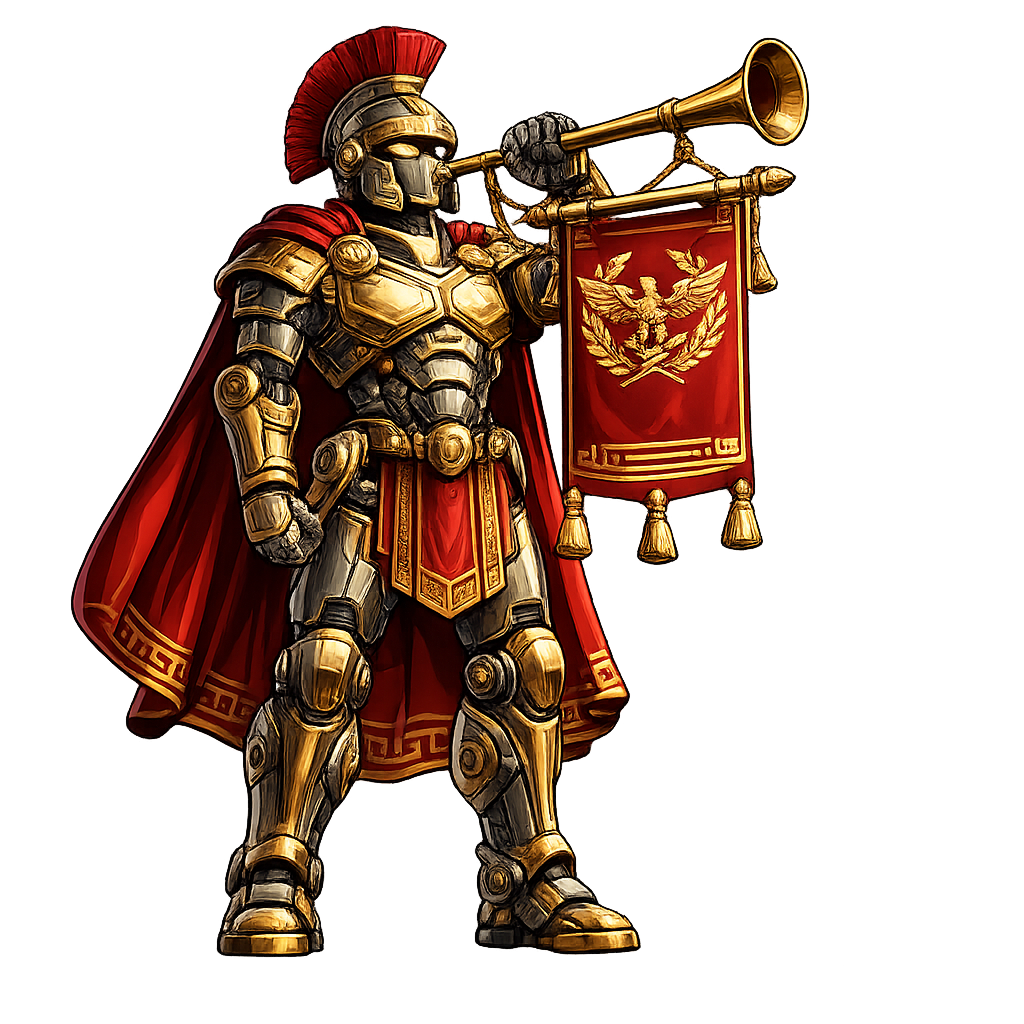
\includegraphics[width=\linewidth]{imagenes/Heraldo_robotico.png}

	\label{fig:Heraldo_robotico}
\end{minipage}
\hfill
\begin{minipage}[c]{0.55\textwidth}
\begin{center}
		\textbf{{\LARGE PRAECO}}
\end{center}
	\textit{Los praecones (singular: \textbf{praeco}) eran los heraldos oficiales en la Antigua Roma. Su función era ser la "voz pública" del Estado.}
\end{minipage}

\section{Propuesta y objetivos}

El objetivo general de este Trabajo Fin de Máster es diseñar, desarrollar y evaluar un sistema móvil de asistencia para personas con discapacidad visual o baja visión, denominado \textit{Praeco}, capaz de reconocer información textual presente en el etiquetado de productos, mejorar de forma conservadora los errores producidos durante el reconocimiento OCR, detectar posibles alérgenos y comunicar la información obtenida mediante síntesis de voz.

Como resultado de la evolución del proyecto, Praeco se ha estructurado en un ecosistema formado por tres aplicaciones independientes pero relacionadas entre sí: \textbf{Praeco Desarrollo}, \textbf{Praeco Usuario} y \textbf{Praeco Análisis}. Esta separación permite diferenciar claramente las funciones de desarrollo, aprendizaje y evaluación experimental de aquellas necesarias para el funcionamiento de la aplicación destinada al usuario final.

Los objetivos específicos del proyecto son los siguientes:

\begin{itemize}
	
	\item Diseñar e implementar una arquitectura de procesamiento capaz de adquirir imágenes mediante la cámara del dispositivo móvil, seleccionar una región de interés y evaluar automáticamente su calidad mediante parámetros de nitidez, brillo y contraste.
	
	\item Estudiar la optimización de la captura automática mediante análisis previo de fotogramas, iluminación auxiliar y mejora condicional del contraste con CLAHE.

\item Integrar un motor de reconocimiento óptico de caracteres basado en Google ML Kit que permita obtener el texto presente en etiquetas y otros soportes impresos utilizando un dispositivo Android convencional.
	
	\item Desarrollar un sistema híbrido y conservador de corrección de errores OCR basado en distancia de Levenshtein, semejanza fonética, diccionarios lingüísticos, reglas de protección, vocabulario adaptativo y mecanismos de aprendizaje incremental.
	
	\item Implementar mecanismos de filtrado y reconstrucción del texto reconocido que permitan reducir información irrelevante y preparar los tokens para las etapas posteriores de corrección y análisis.
	
	\item Incorporar un módulo de detección de alérgenos capaz de identificar términos asociados a gluten, lácteos, huevo, frutos secos, cacahuete, soja, pescado y marisco, considerando además determinadas expresiones de ausencia, como \textit{«sin gluten»}, con el objetivo de reducir falsos positivos.
	
	\item Proporcionar una salida accesible mediante síntesis de voz (\textit{Text-to-Speech}, TTS), de forma que el texto reconocido, corregido y las advertencias generadas puedan ser comunicados auditivamente al usuario.
	
	\item Desarrollar \textbf{Praeco Desarrollo} como aplicación destinada a la experimentación y evolución del sistema. Esta versión incorpora las funciones de captura, OCR, corrección, detección de alérgenos y TTS, junto con mecanismos específicos de introducción del \textit{ground truth}, aprendizaje adaptativo, trazabilidad, almacenamiento de experimentos y evaluación cuantitativa mediante CER y WER.
	
	\item Implementar en Praeco Desarrollo un sistema de aprendizaje incremental capaz de registrar asociaciones entre errores OCR y palabras correctas, controlar su frecuencia y posibles conflictos, y generar progresivamente un diccionario adaptativo con vocabulario válido aprendido durante la fase experimental.
	
	\item Desarrollar \textbf{Praeco Usuario} como una aplicación independiente destinada al uso normal del asistente. Esta versión utiliza los recursos lingüísticos previamente aprendidos y congelados, conservando únicamente las funciones necesarias para el usuario: cámara, evaluación de calidad, OCR, filtrado, corrección, detección de alérgenos y síntesis de voz, sin incorporar \textit{ground truth}, aprendizaje ni herramientas de evaluación experimental.
	
	\item Desarrollar \textbf{Praeco Análisis} como una tercera aplicación independiente destinada al tratamiento de los resultados experimentales generados por Praeco Desarrollo. Esta aplicación permite seleccionar el fichero de experimentos y realizar el análisis estadístico de las métricas CER y WER, la mejora producida por el corrector, los tiempos de procesamiento, las variables de calidad de imagen, los casos de mejora y empeoramiento y la separación entre experimentos de aprendizaje y validación.
	
	\item Evaluar objetivamente el funcionamiento del sistema mediante las métricas \textit{Character Error Rate} (CER) y \textit{Word Error Rate} (WER), comparando el texto producido originalmente por el OCR con el obtenido después de aplicar el corrector de Praeco.
	
	\item Analizar el coste computacional de las principales etapas del procesamiento mediante el registro de los tiempos de captura, reconocimiento OCR, corrección y detección de alérgenos, permitiendo estudiar la viabilidad del sistema para su utilización interactiva en un dispositivo móvil.
	
	\item Establecer una metodología experimental que mantenga separados los procesos de aprendizaje y validación. Una vez estabilizados el código y los recursos lingüísticos, estos se congelan para realizar una validación independiente, evitando que los datos empleados durante el aprendizaje condicionen los resultados finales.
	
	\item Diseñar una interfaz sencilla y accesible, orientada a reducir la dependencia de elementos exclusivamente visuales y favorecer la interacción mediante información auditiva.
	
\end{itemize}

La arquitectura resultante establece, por tanto, una separación funcional entre las tres aplicaciones. \textbf{Praeco Desarrollo} permite construir, aprender y evaluar el sistema; \textbf{Praeco Usuario} constituye el asistente operativo destinado al usuario final utilizando recursos previamente validados; y \textbf{Praeco Análisis} proporciona las herramientas necesarias para estudiar estadísticamente los resultados experimentales. Esta división facilita la trazabilidad del proceso de desarrollo y permite realizar una evaluación metodológicamente independiente del sistema antes de transferir los recursos validados a la aplicación de usuario.
% ------------------------------------------------
% ESTADO DEL ARTE
% ------------------------------------------------

\chapter{Estado del Arte}

La asistencia tecnológica destinada a personas con discapacidad visual ha evolucionado desde dispositivos específicos hacia soluciones basadas en teléfonos móviles, visión artificial y procesamiento local o remoto de la información. El objetivo común de estas tecnologías es aumentar la autonomía del usuario ante tareas cotidianas como la lectura de documentos, la identificación de productos o el acceso a información textual. La literatura sobre tecnología asistencial destaca la importancia de combinar funcionalidad, accesibilidad y facilidad de uso en este tipo de sistemas \cite{assistive}.

En el ámbito del procesamiento de imágenes, las técnicas de visión artificial permiten adquirir, mejorar y analizar imágenes capturadas en condiciones reales \cite{gonzalez,mobilevision}. Sobre esta base, el reconocimiento óptico de caracteres (OCR) transforma el contenido visual en texto susceptible de ser procesado posteriormente. Los motores OCR modernos ofrecen resultados útiles en numerosos escenarios, aunque su precisión continúa dependiendo de factores como el enfoque, la iluminación, el contraste, la perspectiva, el tamaño de los caracteres y la disposición del texto \cite{ocr}.

La corrección posterior al OCR constituye, por tanto, una etapa relevante cuando se trabaja con imágenes no controladas. Entre las técnicas clásicas se encuentra la distancia de Levenshtein, que cuantifica el número mínimo de inserciones, eliminaciones y sustituciones necesarias para transformar una cadena en otra \cite{levenshtein}. Esta medida puede combinarse con información fonética, reglas lingüísticas y modelos de contexto. Los modelos basados en n-gramas permiten representar regularidades locales del lenguaje y constituyen una herramienta habitual dentro del procesamiento del lenguaje natural \cite{nlp}.

Para evaluar cuantitativamente un sistema OCR resulta necesario comparar el texto reconocido con una referencia o \textit{ground truth}. En este trabajo se emplean principalmente el \textit{Character Error Rate} (CER) y el \textit{Word Error Rate} (WER), métricas derivadas de las operaciones de edición necesarias para transformar la hipótesis reconocida en la referencia. Junto con estas métricas de precisión, el tiempo de procesamiento resulta relevante para valorar la viabilidad de una solución interactiva.

% ------------------------------------------------
\section{Soluciones de asistencia visual}
% ------------------------------------------------

Existen aplicaciones comerciales que demuestran la utilidad de la visión artificial y el OCR como tecnologías de apoyo. \textit{Seeing AI}, desarrollada por Microsoft, integra funciones destinadas a interpretar información visual y textual para usuarios con discapacidad visual \cite{seeingai}. Por su parte, \textit{Google Lens} combina reconocimiento visual y procesamiento de texto dentro del ecosistema de Google \cite{googlelens}. Estas soluciones muestran el potencial de los dispositivos móviles como plataforma de asistencia, aunque su propósito es general y no coincide necesariamente con el flujo específico de captura, corrección léxica, evaluación experimental y detección de términos asociados a alérgenos desarrollado en Praeco.

Desde el punto de vista de la plataforma, Android proporciona acceso a cámara, almacenamiento y servicios de accesibilidad \cite{android}. Flutter y Dart permiten construir una aplicación móvil multiplataforma a partir de una base de código común \cite{flutter,dart}. En Praeco se ha empleado Google ML Kit para realizar el reconocimiento óptico de caracteres en el dispositivo \cite{mlkit}, junto con síntesis de voz para comunicar los resultados al usuario.

% ------------------------------------------------
\section{Tecnologías relevantes para Praeco}
% ------------------------------------------------

\subsection{Reconocimiento óptico de caracteres}

El OCR constituye el núcleo de la extracción textual. En un escenario de etiquetado de productos, la entrada no procede de documentos digitalizados en condiciones controladas, sino de fotografías realizadas con un teléfono móvil. Por ello, la calidad de la captura condiciona directamente el texto obtenido. Praeco incorpora una etapa previa de evaluación de nitidez, brillo y contraste para reducir la probabilidad de procesar imágenes claramente inadecuadas.

\subsection{Corrección léxica posterior al OCR}

La salida del OCR puede contener sustituciones, inserciones, eliminaciones o segmentaciones incorrectas. Praeco aborda este problema mediante un corrector conservador que combina distancia de Levenshtein \cite{levenshtein}, similitud fonética, criterios dependientes de la longitud, reglas de protección y recursos léxicos. El objetivo no es modificar sistemáticamente el texto reconocido, sino intervenir únicamente cuando existe evidencia suficiente para proponer una alternativa más fiable.

El proyecto contempla asimismo recursos de contexto basados en n-gramas. No obstante, aunque dichos recursos se encuentran disponibles en la implementación, la corrección contextual mediante n-gramas no forma parte de la ruta activa utilizada en la evaluación final. Esta distinción es importante para no atribuir a ese mecanismo las mejoras cuantitativas presentadas posteriormente.

\subsection{Procesamiento local y privacidad}

La ejecución en el propio dispositivo reduce la necesidad de transmitir imágenes de etiquetas a servicios externos y disminuye la dependencia de conectividad. Esta característica resulta especialmente relevante en una aplicación asistencial que puede utilizarse en contextos cotidianos y con información capturada directamente por la cámara. La arquitectura final de Praeco está orientada a Android y utiliza componentes locales para las etapas principales de captura, OCR, corrección, detección y síntesis de voz.

% ------------------------------------------------
\section{Praeco y su aportación}
% ------------------------------------------------

Praeco se plantea como un prototipo experimental y asistencial centrado en el acceso a información textual presente en etiquetas. A diferencia de una herramienta OCR genérica, integra en un mismo flujo la adquisición de la imagen, su evaluación de calidad, la selección de una región de interés, el reconocimiento mediante ML Kit, el filtrado y reconstrucción del texto, la corrección léxica, la detección de términos asociados a alérgenos y la síntesis de voz.

El corrector protege números, cantidades, palabras cortas, términos previamente validados y otras expresiones que no deben modificarse sin evidencia suficiente. Durante la fase de desarrollo se incorpora además aprendizaje adaptativo a partir de errores observados y validados. Para la evaluación final, estos recursos se congelan, evitando que las muestras de validación modifiquen simultáneamente el conocimiento utilizado por el corrector.

La Tabla~\ref{tab:comparativa_ocr} resume, de forma cualitativa, algunas diferencias entre soluciones de propósito general y el enfoque específico adoptado en Praeco. La comparación pretende contextualizar funcionalidades y no establecer una clasificación de precisión, ya que no se ha realizado un ensayo experimental común entre las aplicaciones.

\begin{table}[htbp]
    \centering
    \caption{Comparación cualitativa entre soluciones de asistencia visual y Praeco.}
    \label{tab:comparativa_ocr}
    \renewcommand{\arraystretch}{1.25}
    \begin{tabularx}{\textwidth}{@{}lXXXX@{}}
        \toprule
        \textbf{Sistema} & \textbf{OCR} & \textbf{Orientación} & \textbf{Corrección propia evaluada} & \textbf{Alérgenos} \\
        \midrule
        Seeing AI \cite{seeingai} & Sí & Asistencia visual general & No evaluada en este TFM & No específica \\
        Google Lens \cite{googlelens} & Sí & Búsqueda y análisis visual general & No evaluada en este TFM & No específica \\
        \textbf{Praeco} & \textbf{Sí} & \textbf{Etiquetado y accesibilidad} & \textbf{Sí} & \textbf{Detección de términos} \\
        \bottomrule
    \end{tabularx}
\end{table}

La comparación pone de manifiesto que la aportación principal de Praeco no consiste en competir con plataformas comerciales de visión artificial de propósito general, sino en estudiar de forma reproducible una cadena concreta de procesamiento y evaluar cuantitativamente el efecto de la corrección posterior al OCR. La arquitectura separa además el entorno de desarrollo y aprendizaje, la aplicación destinada al usuario y la herramienta de análisis experimental.

% ------------------------------------------------
\section{Brecha abordada por el trabajo}
% ------------------------------------------------

A partir del análisis anterior, el presente TFM aborda una combinación de necesidades: ejecución sobre un dispositivo móvil comercial, control explícito de la calidad de captura, corrección léxica conservadora, aprendizaje adaptativo durante el desarrollo, detección de términos asociados a alérgenos, salida accesible mediante voz y evaluación cuantitativa mediante CER, WER y tiempos de procesamiento.

El interés del trabajo reside, por tanto, tanto en el prototipo funcional como en la metodología experimental utilizada para estudiar sus limitaciones. Los capítulos siguientes describen la arquitectura de Praeco, los mecanismos implementados y la evaluación realizada con los recursos de aprendizaje congelados.

% ------------------------------------------
% Tema 3 Materiales y Métodos 
% ------------------------------------------

\chapter{Materiales y métodos}

\section{Arquitectura de la aplicación y funcionamiento detallado de Praeco}

Praeco es un asistente accesible para dispositivos Android orientado a personas con discapacidad visual o baja visión. Su objetivo es utilizar la cámara del teléfono y técnicas de visión artificial para reconocer el texto presente en el etiquetado de productos, corregir de forma conservadora determinados errores producidos durante el reconocimiento OCR, identificar posibles alérgenos y comunicar el resultado mediante síntesis de voz.

En la arquitectura actual se distinguen tres aplicaciones: \textbf{Praeco Desarrollo}, utilizada para la experimentación, aprendizaje, trazabilidad y evaluación; \textbf{Praeco Usuario}, que constituye la aplicación operativa final con los recursos aprendidos congelados; y \textbf{Praeco Análisis}, destinada al tratamiento estadístico de los resultados almacenados por la versión de Desarrollo.

\begin{figure}[htbp]
	\centering
	\resizebox{0.98\textwidth}{!}{%
		\begin{tikzpicture}[
			box/.style={
				draw,
				rounded corners,
				align=center,
				minimum width=4.1cm,
				minimum height=1.15cm,
				font=\small
			},
			line/.style={
				-{Latex[length=2.5mm]},
				thick
			}
			]
			
			% Nodo principal
			\node[box] (eco) {ECOSISTEMA PRAECO};
			
			% Tres aplicaciones
			\node[
			box,
			below left=2.0cm and 5.5cm of eco
			] (dev) {
				PRAECO DESARROLLO\\
				Captura, OCR, corrección\\
				alérgenos, TTS, aprendizaje\\
				CER/WER y trazabilidad
			};
			
			\node[
			box,
			below=2.0cm of eco
			] (usr) {
				PRAECO USUARIO\\
				Captura, OCR, corrección\\
				alérgenos y TTS\\
				sin aprendizaje ni evaluación
			};
			
			\node[
			box,
			below right=2.0cm and 5.5cm of eco
			] (ana) {
				PRAECO ANÁLISIS\\
				Lectura de experimentos\\
				estadísticas y comparación\\
				de resultados
			};
			
			% Flechas separadas
			\draw[line]
			(eco.south west) -- (dev.north);
			
			\draw[line]
			(eco.south) -- (usr.north);
			
			\draw[line]
			(eco.south east) -- (ana.north);
			
			% Comunicación Desarrollo -> Análisis
			\draw[line]
			(dev.south) -- ++(0,-1.0cm)
			-| node[
			pos=0.5,
			below,
			font=\scriptsize
			] {\texttt{experimentos.csv}}
			(ana.south);
			
		\end{tikzpicture}%
	}
	
	\caption{Arquitectura general del ecosistema Praeco.}
	\label{fig:ecosistema-praeco}
\end{figure}

Como se muestra en la Figura~\ref{fig:ecosistema-praeco}, el ecosistema se divide en tres aplicaciones con responsabilidades diferenciadas. Esta separación resulta importante metodológicamente: Praeco Desarrollo permite desarrollar, aprender y evaluar el sistema; Praeco Usuario representa la aplicación destinada al uso normal; y Praeco Análisis estudia experimentalmente los resultados obtenidos.

\subsection{Flujo general de procesamiento}

El funcionamiento principal de Praeco sigue una cadena secuencial: adquisición de la imagen, selección de la región de interés, evaluación de calidad, reconocimiento OCR, filtrado, reconstrucción y protección de tokens, corrección léxica, detección de alérgenos y síntesis de voz.

\begin{figure}[htbp]
\centering
\resizebox{0.93\textwidth}{!}{%
\begin{tikzpicture}[node distance=0.43cm,
 box/.style={draw,rounded corners,align=center,minimum width=6.4cm,minimum height=0.64cm,font=\small},
 line/.style={-{Latex[length=2mm]},thick}]
 \node[box] (cam) {Cámara: análisis de fotogramas en vista previa};
 \node[box,below=of cam] (luz) {Brillo inferior a 150: linterna continua y estabilización};
 \node[box,below=of luz] (cal) {Evaluación de nitidez, brillo y contraste};
 \node[box,below=of cal] (cap) {Captura automática de una fotografía y recorte ROI};
 \node[box,below=of cap] (mej) {Mejora condicional: CLAHE o ajuste de iluminación};
 \node[box,below=of mej] (sel) {OCR original / OCR procesado cuando procede; selección};
 \node[box,below=of sel] (fil) {Filtrado y reconstrucción de tokens};
 \node[box,below=of fil] (cor) {Corrección léxica conservadora};
 \node[box,below=of cor] (out) {Detección de alérgenos y síntesis de voz};
 \foreach \a/\b in {cam/luz,luz/cal,cal/cap,cap/mej,mej/sel,sel/fil,fil/cor,cor/out}{\draw[line] (\a)--(\b);}
\end{tikzpicture}}
\caption{Flujo de captura rápida y preprocesamiento condicional de Praeco. La captura se realiza al cumplir los criterios de calidad; la linterna permanece encendida hasta finalizarla cuando es necesaria.}
\label{fig:flujo-principal-praeco}
\end{figure}

La Figura~\ref{fig:flujo-principal-praeco} resume el flujo de procesamiento desde la captura hasta la obtención y comunicación del resultado.

\subsection{Adquisición de la imagen y región de interés}

El procesamiento comienza con la cámara del teléfono móvil. La cámara proporciona imágenes de la etiqueta situada delante del dispositivo. El objetivo no es únicamente tomar una fotografía, sino obtener una captura que presente condiciones suficientemente buenas para realizar posteriormente el reconocimiento OCR.

En la versión optimizada, Praeco analiza fotogramas de la vista previa antes de efectuar una única fotografía. La decisión automática se basa en la estabilidad de la imagen y en estimaciones de nitidez, brillo y contraste. Se evita así adquirir y reconocer mediante OCR tres fotografías sucesivas para escoger una de ellas, operación que aumentaba la latencia. Cuando la imagen no reúne los criterios establecidos, la aplicación continúa evaluando la vista previa hasta obtener condiciones apropiadas.

Una vez realizada la captura, Praeco recorta una \textit{Region of Interest} (ROI), que delimita la zona de la imagen que interesa procesar. En la implementación se conserva todo el ancho y aproximadamente los dos tercios superiores de la imagen. Esta reducción permite limitar la presencia de fondo y de elementos que no pertenecen al etiquetado, al mismo tiempo que disminuye el volumen de información que debe procesarse.

La imagen correspondiente a la ROI constituye la entrada del motor OCR. Se conserva una copia original y, cuando las condiciones lo requieren, se genera otra con mejora de imagen. El reconocimiento se aplica inicialmente a la imagen original y puede compararse con el de la procesada, seleccionando la alternativa mediante los criterios de puntuación programados.

\subsection{Evaluación de la calidad de imagen}

Antes de aceptar una captura, Praeco analiza tres propiedades principales: \textbf{nitidez}, \textbf{brillo} y \textbf{contraste}. La nitidez permite estimar si la fotografía está correctamente enfocada y se calcula mediante la varianza de la respuesta de un operador Laplaciano. El brillo representa el nivel medio de luminancia, mientras que el contraste representa la dispersión de los niveles de luminancia.

La luminancia se aproxima mediante
\begin{equation}
	L=0{,}299R+0{,}587G+0{,}114B.
\end{equation}

\begin{figure}[htbp]
	\centering
	\resizebox{0.98\textwidth}{!}{%
		\begin{tikzpicture}[node distance=1cm and 1cm,
			box/.style={draw, rounded corners, align=center, minimum width=3.1cm, minimum height=0.8cm, font=\small},
			line/.style={-{Latex[length=2mm]}, thick}]
			\node[box] (img) {Imagen ROI};
			\node[box, below left=1cm and 2.6cm of img] (nit) {Nitidez\\Varianza Laplaciana};
			\node[box, below=1cm of img] (bri) {Brillo\\Luminancia media};
			\node[box, below right=1cm and 2.6cm of img] (con) {Contraste\\Desviación típica};
			\node[box, below=2.5cm of img] (eval) {Evaluación de calidad};
			\node[box, below left=1cm and 1.8cm of eval] (repeat) {Repetir};
			\node[box, below right=1cm and 1.8cm of eval] (accept) {Aceptar};
			\draw[line](img)--(nit); \draw[line](img)--(bri); \draw[line](img)--(con);
			\draw[line](nit)--(eval); \draw[line](bri)--(eval); \draw[line](con)--(eval);
			\draw[line](eval)--(repeat); \draw[line](eval)--(accept);
		\end{tikzpicture}%
	}
	\caption{Evaluación de calidad de la imagen.}
	\label{fig:calidad-praeco}
\end{figure}

La Figura~\ref{fig:calidad-praeco} representa las variables utilizadas para decidir si la imagen presenta unas condiciones mínimas de calidad. Los umbrales básicos de aceptación son nitidez mínima 100, contraste mínimo 20, brillo mínimo 35 y brillo máximo 225. Estos umbrales de aceptación se distinguen del umbral de activación de la linterna (brillo inferior a 150) y del criterio de CLAHE (contraste inferior a 25). Estos valores son parámetros iniciales del prototipo y no deben interpretarse como límites universalmente validados. Una imagen puede superar dichos umbrales y producir un OCR deficiente debido a la perspectiva, curvatura del envase, reflejos, tipografía, tamaño de letra o disposición del texto.

\subsection{Control automático de iluminación y estabilización}

La versión optimizada incorpora control de la iluminación auxiliar a partir de la luminancia estimada en la vista previa. Se ha fijado experimentalmente un umbral de activación de \textbf{150} en la escala de brillo de 0 a 255. Cuando la iluminación es inferior, se solicita al controlador de cámara el modo \texttt{FlashMode.torch}, que proporciona iluminación continua en lugar de un destello sincronizado con la fotografía. Una vez encendida, la linterna permanece activa durante la evaluación y la adquisición, incluso si el brillo aumenta por efecto de la propia luz. Esta retención evita la oscilación encendido--apagado observada durante el desarrollo.

Tras la activación se introduce una espera aproximada de \textbf{900~ms} para permitir la estabilización de la exposición y el enfoque. Finalizada la captura, se apaga la linterna. El umbral de 150 y el tiempo de espera son parámetros de ingeniería ajustados durante las pruebas del prototipo, no constantes óptimas universales: pueden depender de la cámara, la distancia y la reflectancia del envase.

\subsection{Preprocesamiento condicional mediante CLAHE}

Se ha añadido un módulo opcional de mejora de imagen previo al OCR. Su objetivo es actuar únicamente cuando la calidad de la captura lo justifique, conservando la imagen original como referencia. En particular, si el contraste medido es inferior a un umbral operativo de \textbf{25}, se puede aplicar \textit{Contrast Limited Adaptive Histogram Equalization} (CLAHE), una ecualización adaptativa del histograma limitada para reducir la amplificación excesiva del ruido.

El procedimiento divide la imagen en regiones locales, calcula sus histogramas de luminancia, limita las frecuencias excesivas y redistribuye los valores de intensidad; la interpolación entre regiones reduce las discontinuidades de contraste. Si el problema dominante es la iluminación, se contempla un ajuste de brillo. Cuando la imagen ya presenta condiciones suficientes, no se aplica mejora adicional. CLAHE no corrige por sí mismo el desenfoque ni garantiza una disminución del error OCR.

La interfaz de resultados presenta la fotografía original y, cuando se ha generado, la procesada, junto con la indicación del tratamiento utilizado (CLAHE, ajuste de iluminación o ninguno) y la procedencia de la imagen elegida para el reconocimiento. Esta comparación visual permite comprobar el efecto de la mejora sin confundirlo con una ganancia de precisión demostrada.

La selección entre resultados OCR se efectúa mediante la puntuación prevista en la implementación y no mediante el \textit{ground truth}, que se reserva para la evaluación experimental. La incorporación de CLAHE debe evaluarse mediante un ensayo de ablación con imágenes idénticas y los mismos recursos lingüísticos congelados.

\subsection{Reconocimiento OCR mediante Google ML Kit}

Una vez aceptada la imagen, se procesa mediante \texttt{TextRecognizer} de Google ML Kit. La salida inicial constituye el \textbf{OCR bruto}. Esta salida puede contener sustituciones de caracteres visualmente parecidos, errores de separación, puntuación o reconocimiento de palabras. Por ello, ML Kit constituye la primera etapa del reconocimiento textual, pero no el resultado definitivo utilizado por Praeco.

\subsection{Filtrado del OCR}

El texto bruto pasa por una etapa de filtrado cuyo objetivo es eliminar información que no resulta útil para el análisis y reducir la interferencia de determinados elementos comerciales o auxiliares. El filtro trabaja por líneas y puede descartar URL, cadenas exclusivamente numéricas, determinados códigos largos, identificadores de lote, cantidades aisladas con unidades y ciertas expresiones de reciclaje. Las líneas que contienen información textual útil se conservan para las etapas posteriores.

Debe distinguirse entre \textbf{OCR bruto}, \textbf{OCR filtrado} y \textbf{texto corregido}. El primero es la salida directa del motor OCR; el segundo es el resultado de aplicar las reglas de limpieza; y el tercero incorpora el postprocesamiento léxico de Praeco.

\subsection{Reconstrucción y protección de tokens}

Tras el filtrado, el texto se representa como una secuencia de palabras o \textit{tokens}. Esta representación permite analizar cada palabra antes de decidir si debe mantenerse o corregirse. Praeco incorpora además mecanismos para reconstruir determinadas separaciones o uniones anómalas producidas por el OCR.

Uno de los principios del corrector es que una palabra desconocida no debe corregirse automáticamente. Antes de aplicar una corrección se comprueba si el token pertenece a alguna categoría protegida: números y cantidades, palabras muy cortas, \textit{stopwords}, vocabulario presente en el diccionario base o adaptativo, determinados términos ingleses y nombres propios explícitamente protegidos.

Esta protección es especialmente relevante en etiquetas multilingües. Por ejemplo, la palabra italiana \textit{bianco} puede aparecer realmente en una etiqueta y, si forma parte del vocabulario válido aprendido, debe conservarse. El objetivo del corrector no es traducir ni castellanizar el etiquetado, sino corregir errores atribuibles al OCR.

\subsection{Corrector léxico híbrido}

Cuando un token no está protegido, Praeco genera candidatos a partir del diccionario base, del diccionario adaptativo y de los recursos léxicos disponibles. Cada candidato se evalúa combinando distancia de edición, semejanza fonética y diferencia de longitud. Si el mejor candidato no alcanza una confianza suficiente o existe ambigüedad entre candidatos, se conserva la palabra original.

\begin{figure}[htbp]
	\centering
	\resizebox{0.98\textwidth}{!}{%
		\begin{tikzpicture}[node distance=0.65cm,
			box/.style={draw, rounded corners, align=center, minimum width=5.6cm, minimum height=0.75cm, font=\small},
			line/.style={-{Latex[length=2.2mm]}, thick}]
			\node[box] (tok) {Token OCR no protegido};
			\node[box, below=of tok] (cand) {Generación de candidatos: diccionario base, adaptativo y léxico};
			\node[box, below=of cand] (score) {Puntuación: Levenshtein + fonética + diferencia de longitud};
			\node[box, below=of score] (conf) {Evaluación de umbral, distancia relativa y ambigüedad};
			\node[box, below left=1.7cm and 0.2cm of conf] (keep) {Conservar original};
			\node[box, below right=1.7cm and 0.2cm of conf] (corr) {Aceptar corrección};
			\draw[line](tok)--(cand); \draw[line](cand)--(score); \draw[line](score)--(conf);
			\draw[line](conf)--(keep); \draw[line](conf)--(corr);
		\end{tikzpicture}%
	}
	\caption{Proceso de decisión del corrector léxico de Praeco.}
	\label{fig:corrector-praeco}
\end{figure}

La lógica general de decisión del corrector se sintetiza en la Figura~\ref{fig:corrector-praeco}.

\subsection{Distancia de Levenshtein}

La Distancia de Levenshtein es uno de los algoritmos más utilizados en procesamiento del lenguaje natural (NLP), corrección ortográfica y sistemas OCR para medir la similitud entre dos palabras. 

La distancia de Levenshtein mide el número mínimo de operaciones necesarias para transformar una cadena en otra mediante inserciones, eliminaciones y sustituciones. Por ejemplo, transformar \texttt{lechf} en \texttt{leche} requiere una sustitución, por lo que su distancia es uno. Una distancia pequeña indica elevada similitud ortográfica, pero Praeco no utiliza este valor de forma aislada: se combina con otros criterios para evitar correcciones agresivas.

Los límites de distancia dependen de la longitud de la palabra: para tokens de longitud menor o igual que cinco se admite como máximo una distancia ponderada de 1; hasta ocho caracteres, 2; y para longitudes superiores, 3. Además se aplica un límite relativo y criterios de confianza y separación entre candidatos.

\subsection{Información fonética}

La semejanza fonética complementa la semejanza ortográfica. La función de fonetización agrupa algunas grafías potencialmente confundibles y permite penalizar candidatos que, aunque sean próximos gráficamente, resulten menos plausibles desde el punto de vista fonético. La decisión final combina ambas fuentes de información con la diferencia de longitud.

\subsection{Diccionario adaptativo y aprendizaje incremental}

Praeco Desarrollo incorpora un mecanismo de aprendizaje basado en dos recursos diferentes. El fichero \texttt{errores\_ocr.json} registra asociaciones observadas entre formas reconocidas erróneamente y palabras correctas, junto con su frecuencia y estado. El fichero \texttt{diccionario\_adaptativo.json}, en cambio, contiene vocabulario válido aprendido y no una tabla de errores.

Cuando el modo de aprendizaje está activo, el texto OCR se alinea con el texto real o \textit{ground truth}. Las asociaciones próximas se registran y aumentan su frecuencia cuando vuelven a observarse. Las asociaciones suficientemente repetidas, válidas y no conflictivas pueden integrarse en el diccionario adaptativo. En la implementación actual, la integración exige una frecuencia mínima de tres observaciones.

\medskip

\begin{figure}[htbp]
	\centering
	\resizebox{0.72\textwidth}{!}{%
		\begin{tikzpicture}[node distance=0.6cm,
			box/.style={draw, rounded corners, align=center, minimum width=5.5cm, minimum height=0.20cm, font=\small},
			line/.style={-{Latex[length=1.2mm]}, thick}]
			\node[box] (ocr) {OCR original + texto real (ground truth)};
			\node[box, below=of ocr] (ali) {Alineación y comparación de palabras};
			\node[box, below=of ali] (err) {Registro de asociación en \texttt{errores\_ocr.json}};
			\node[box, below=of err] (freq) {Incremento de frecuencia y control de conflictos};
			\node[box, below=of freq] (dic) {Integración de palabra válida en \texttt{diccionario\_adaptativo.json}};
			\draw[line](ocr)--(ali); \draw[line](ali)--(err); \draw[line](err)--(freq); \draw[line](freq)--(dic);
		\end{tikzpicture}%
	}
	\caption{Esquema del aprendizaje incremental de Praeco Desarrollo.}
	\label{fig:aprendizaje-praeco}
\end{figure}

La Figura~\ref{fig:aprendizaje-praeco} muestra la secuencia seguida durante el aprendizaje incremental, desde la comparación con el texto de referencia hasta la posible incorporación de vocabulario validado.

\medskip

Por ejemplo, si el OCR produce repetidamente \textit{biarico} mientras el texto real contiene \textit{bianco}, la asociación puede registrarse como error. En cambio, \textit{bianco} puede incorporarse al diccionario adaptativo como palabra válida. De esta forma, el sistema aprende vocabulario del dominio sin considerar erróneas palabras extranjeras que realmente aparecen en el etiquetado.

\subsection{Corrección contextual mediante n-gramas}

El proyecto dispone de recursos de unigramas, bigramas, trigramas y cuatrigramas relacionados con el dominio alimentario. Estos recursos permiten representar secuencias frecuentes como \textit{aceite de}, \textit{harina de}, \textit{puede contener} o \textit{trazas de}. El contexto puede reforzar una corrección que resulte coherente con las palabras vecinas.

No obstante, en la validación congelada utilizada para los resultados finales debe indicarse expresamente si la llamada a la corrección contextual está activa o desactivada. Cuando se encuentra desactivada, los resultados corresponden al OCR y al corrector léxico activo y no constituyen una evaluación de la corrección contextual por n-gramas.

\subsection{Detección de alérgenos}

El texto corregido se utiliza como entrada del detector de alérgenos. La implementación contempla las categorías gluten, lácteos, huevo, frutos secos, cacahuete, soja, pescado y marisco mediante un conjunto de términos configurados para cada una de ellas. El sistema analiza la presencia de estos términos en el texto reconocido y, cuando identifica una coincidencia positiva, genera un aviso del tipo \textit{«Atención: contiene ...»}.

Para reducir la aparición de falsos positivos, Praeco no considera únicamente la presencia aislada del nombre de un alérgeno, sino que tiene en cuenta determinadas expresiones que indican explícitamente su ausencia. De este modo, una aparición de la palabra \textit{gluten} no implica necesariamente que el producto contenga gluten. Si el texto reconocido contiene expresiones como \textit{«sin gluten»}, \textit{«libre de gluten»} o construcciones equivalentes contempladas por las reglas implementadas, el sistema interpreta que dicha mención corresponde a una declaración de ausencia y evita generar una alerta positiva para ese alérgeno. El mismo criterio puede aplicarse a otras categorías cuando aparecen asociadas a expresiones de exclusión reconocidas por el sistema.

Por tanto, el proceso de detección puede representarse mediante dos niveles de comprobación. En primer lugar, se localizan los términos asociados a las distintas categorías de alérgenos y, posteriormente, se comprueba si la aparición se encuentra dentro de una expresión de exclusión. Si existe una coincidencia positiva y no está afectada por una regla de ausencia, Praeco genera el mensaje \textit{«Atención: contiene ...»}. Si no se detectan términos configurados como alérgenos, o las apariciones encontradas corresponden únicamente a expresiones explícitas de ausencia reconocidas por el sistema, se informa mediante el mensaje \textit{«No se detectan alérgenos»}.

Este tratamiento resulta especialmente importante en el etiquetado alimentario, ya que expresiones como \textit{«sin gluten»} contienen literalmente el término que identifica al alérgeno. Una búsqueda basada exclusivamente en palabras clave produciría en este caso un falso positivo. La comprobación de expresiones de ausencia permite a Praeco distinguir, dentro de las reglas implementadas, entre una mención positiva y una declaración explícita de exclusión.

No obstante, este mecanismo constituye una ayuda experimental basada en coincidencias léxicas y reglas de contexto local, y no un análisis semántico, nutricional o clínico completo. La expresión \textit{«No se detectan alérgenos»} significa únicamente que, a partir del texto reconocido por el OCR y de las reglas y categorías configuradas en Praeco, no se ha identificado una presencia positiva de los alérgenos considerados. Por ello, este resultado no certifica que el producto esté libre de alérgenos y no debe utilizarse como única fuente para decidir su consumo.

\subsection{Síntesis de voz}

La accesibilidad se completa mediante \textit{Text-to-Speech} (TTS). El texto corregido y los avisos generados se transforman en voz, permitiendo utilizar la aplicación sin depender exclusivamente de la lectura visual de la pantalla. La configuración principal utiliza el idioma \texttt{es-ES}.

La velocidad de reproducción de la síntesis de voz es un parámetro configurable mediante software, lo que permite adaptar el ritmo de lectura a las necesidades y preferencias del usuario. De esta forma, la aplicación puede proporcionar una locución más lenta para facilitar la comprensión o, alternativamente, aumentar la velocidad para usuarios habituados al uso de lectores de pantalla y sistemas de asistencia por voz. Esta posibilidad de configuración contribuye a mejorar la accesibilidad y flexibilidad del sistema, al permitir personalizar la presentación auditiva de la información. La velocidad programada por defecto es 0,5.

\subsection{Evaluación mediante ground truth, CER y WER}

\textbf{Esta funcionalidad está presente solo en Praeco Desarrollo.}

 Durante los experimentos, el usuario introduce el texto real de la etiqueta, que actúa como \textit{ground truth}. La referencia se compara tanto con el OCR original como con el texto corregido.

El \textit{Character Error Rate} (CER) cuantifica el error a nivel de caracteres:
\begin{equation}
	CER=\frac{S+D+I}{N},
\end{equation}
donde $S$ representa sustituciones, $D$ eliminaciones, $I$ inserciones y $N$ el número de caracteres de la referencia.

\medskip

El \textit{Word Error Rate} (WER) utiliza la misma expresión a nivel de palabras:
\begin{equation}
	WER=\frac{S+D+I}{N},
\end{equation}
donde $N$ representa ahora el número de palabras de la referencia. La comparación de \texttt{cer\_ocr} frente a \texttt{cer\_corregido} y de \texttt{wer\_ocr} frente a \texttt{wer\_corregido} permite determinar objetivamente si el corrector mejora, mantiene o empeora el reconocimiento.

\subsection{Medición temporal}

Praeco Desarrollo instrumenta las principales fases del procesamiento mediante temporizadores. Se registran el tiempo de captura $t_{captura}$, el tiempo OCR $t_{OCR}$, el tiempo de corrección $t_{correccion}$ y el tiempo de detección de alérgenos $t_{alergenos}$. El tiempo total analizado puede obtenerse como
\begin{equation}
	t_{total}=t_{captura}+t_{OCR}+t_{correccion}+t_{alergenos}.
\end{equation}

En la versión de captura rápida, la medida de captura debe interpretarse de acuerdo con los puntos de inicio y fin del temporizador: no necesariamente incluye todas las operaciones posteriores de decodificación, recorte y mejora de imagen. Para comparar versiones se recomienda registrar además la latencia completa desde la activación hasta el resultado. Estas medidas permiten evaluar no solo la precisión, sino también el coste computacional y la viabilidad del procesamiento en tiempo real.

\subsection{Almacenamiento experimental}

Praeco Desarrollo crea y en caso de existir actualiza un fichero canónico denominado \texttt{experimentos.csv}. El registro de referencia utilizado para la validación histórica contiene 21 campos:

\begin{center}
	\renewcommand{\arraystretch}{1.3}
	\setlength{\tabcolsep}{12pt}
	\begin{tabular}{lll}
		1. \texttt{fecha}              & 2. \texttt{imagen}              & 3. \texttt{texto\_real} \\
		4. \texttt{ocr}                & 5. \texttt{ocr\_corregido}      & 6. \texttt{cer\_ocr} \\
		7. \texttt{cer\_corregido}     & 8. \texttt{wer\_ocr}            & 9. \texttt{wer\_corregido} \\
		10. \texttt{ancho}             & 11. \texttt{alto}               & 12. \texttt{nitidez} \\
		13. \texttt{brillo}            & 14. \texttt{contraste}          & 15. \texttt{calidad\_aceptable} \\
		16. \texttt{decision\_calidad} & 17. \texttt{t\_captura}         & 18. \texttt{t\_ocr} \\
		19. \texttt{t\_correccion}     & 20. \texttt{t\_alergenos}       & 21. \texttt{modo\_aprendizaje} \\
	\end{tabular}
\end{center}

La instrumentación futura del control de iluminación y del preprocesamiento puede ampliar este esquema con los campos \texttt{brillo\_previo}, \texttt{linterna\_activada}, \texttt{tiempo\_estabilizacion\_ms} y \texttt{mejora\_imagen}. No se presupone que estén presentes en el CSV histórico. Además de este fichero CSV, la versión de Desarrollo conserva información de trazabilidad y recursos de aprendizaje. El campo \texttt{modo\_aprendizaje} permite distinguir las ejecuciones realizadas durante el aprendizaje de aquellas efectuadas con los recursos congelados para validación.

\subsection{Praeco Análisis}

Praeco Análisis constituye una aplicación independiente destinada a procesar el fichero \texttt{experimentos.csv}. El usuario selecciona la ubicación del fichero de experimentos y la aplicación calcula estadísticas globales, compara CER y WER antes y después de la corrección, analiza tiempos de ejecución y permite estudiar las variables de calidad. Esta separación evita incorporar herramientas experimentales innecesarias en la aplicación destinada al usuario final.

\begin{figure}[htbp]
	\centering
	\resizebox{0.98\textwidth}{!}{%
		\begin{tikzpicture}[node distance=0.75cm,
			box/.style={draw, rounded corners, align=center, minimum width=5.2cm, minimum height=0.8cm, font=\small},
			line/.style={-{Latex[length=2.2mm]}, thick}]
			\node[box] (dev) {Praeco Desarrollo};
			\node[box, below=of dev] (csv) {\texttt{experimentos.csv}};
			\node[box, below=of csv] (ana) {Praeco Análisis};
			\node[box, below left=0.8cm and 2.2cm of ana] (cer) {CER / WER};
			\node[box, below=0.8cm of ana] (tim) {Tiempos};
			\node[box, below right=0.8cm and 2.2cm of ana] (qua) {Calidad};
			\node[box, below=2.6cm of ana] (res) {Estadísticas y resultados del TFM};
			\draw[line](dev)--(csv); \draw[line](csv)--(ana); \draw[line](ana)--(cer); \draw[line](ana)--(tim); \draw[line](ana)--(qua);
			\draw[line](cer)--(res); \draw[line](tim)--(res); \draw[line](qua)--(res);
		\end{tikzpicture}%
	}
	\caption{Relación entre Praeco Desarrollo y Praeco Análisis.}
	\label{fig:praeco-analisis}
\end{figure}

La relación entre la aplicación que genera los datos experimentales y la herramienta que los analiza se resume en la Figura~\ref{fig:praeco-analisis}.

\newpage

\subsection{Separación entre Praeco Desarrollo y Praeco Usuario}

La separación entre ambas versiones es fundamental para la metodología experimental. Praeco Desarrollo incorpora \textit{ground truth}, cálculo de CER/WER, aprendizaje, almacenamiento experimental y trazabilidad. Praeco Usuario conserva únicamente las funciones necesarias para el uso normal: cámara, control de calidad, OCR, filtrado, corrección con recursos congelados, detección de alérgenos y TTS.

El procedimiento metodológico consiste en aprender y depurar los recursos en Desarrollo, auditar el \textit{ground truth}, congelar el código y los recursos de aprendizaje, realizar la validación independiente y transferir el diccionario adaptativo validado a la aplicación de Usuario. De este modo, los resultados de aprendizaje no se mezclan con los resultados de validación final.

\begin{figure}[htbp]
	\centering
	\resizebox{0.98\textwidth}{!}{%
		\begin{tikzpicture}[node distance=1cm and 1.3cm,
			box/.style={draw, rounded corners, align=left, text width=6.1cm, minimum height=4.0cm, font=\small},
			line/.style={-{Latex[length=2.2mm]}, thick}]
			\node[box] (dev) {\textbf{PRAECO DESARROLLO}\\[2mm]
				Cámara y calidad\\OCR y filtrado\\Corrección y alérgenos\\TTS\\Ground truth y CER/WER\\Aprendizaje y trazabilidad\\\texttt{experimentos.csv}};
			\node[box, right=of dev] (usr) {\textbf{PRAECO USUARIO}\\[2mm]
				Cámara y calidad\\OCR y filtrado\\Corrección con recursos congelados\\Alérgenos\\TTS\\\textcolor{red}{Sin ground truth}\\\textcolor{red}{Sin aprendizaje ni evaluación}};
			\draw[line] (dev) -- node[above, align=center, font=\scriptsize]{recursos\\congelados} (usr);
		\end{tikzpicture}%
	}
	\caption{Separación funcional entre Praeco Desarrollo y Praeco Usuario.}
	\label{fig:desarrollo-usuario}
\end{figure}

La Figura~\ref{fig:desarrollo-usuario} destaca la separación entre las funciones experimentales de Praeco Desarrollo y la versión destinada al uso normal. En conjunto, Praeco implementa la secuencia \textbf{adquisición de una imagen de calidad $\rightarrow$ reconocimiento OCR $\rightarrow$ filtrado y reconstrucción $\rightarrow$ corrección híbrida $\rightarrow$ detección de alérgenos $\rightarrow$ comunicación accesible mediante voz}. La versión de Desarrollo añade paralelamente aprendizaje, trazabilidad y evaluación cuantitativa mediante CER, WER y tiempos de procesamiento.



%%%%%%%%%%%%%%%%%%%%%%%%%%%%%%%%%%%%%%%%%%%%%%%%%%%%%%%%%%%%%%%%%%%%
\section{Tecnologías y Dependencias Utilizadas}
Las principales bibliotecas y herramientas empleadas son:
\begin{itemize}
	\item \textbf{Flutter}: Framework de UI para el desarrollo de aplicaciones móviles multiplataforma.
	\item \textbf{camera}: Plugin de Flutter para acceder y controlar la cámara del dispositivo.
	\item \textbf{google\_mlkit\_text\_recognition}: Parte de Google ML Kit, utilizada para realizar el reconocimiento óptico de caracteres en las imágenes capturadas.
	\item \textbf{flutter\_tts}: Plugin de Flutter para la funcionalidad de texto a voz (\textit{Text-to-Speech}), permitiendo a la aplicación vocalizar el texto reconocido y corregido.
	\item \textbf{image (package image)}: Biblioteca para el procesamiento de imágenes en Dart, utilizada para recortar las imágenes antes de pasarlas al motor OCR.
	\item \textbf{path\_provider}: Plugin para obtener rutas a directorios comúnmente utilizados en el sistema de archivos.
	\item \textbf{permission\_handler}: Plugin para gestionar los permisos de la aplicación, como el acceso al almacenamiento.
	\item \textbf{google\_mlkit\_language\_id}: Parte de Google ML Kit, utilizada para identificar el idioma del texto detectado y filtrar contenido no relevante.
\end{itemize}

% ------------------------------------------------
% JUSTIFICACION DE LA ELECION DE FLUTTER Y DART
% ------------------------------------------------

\section{Justificación de la elección de Flutter y Dart}

Uno de los aspectos fundamentales durante el desarrollo del sistema fue la selección de las tecnologías software más adecuadas para implementar un asistente inteligente accesible y multiplataforma.

Tras analizar diversas alternativas, se decidió utilizar Flutter junto al lenguaje Dart como base principal del desarrollo.

\begin{itemize}
	
	\item\textbf{Motivo de la elección.} La elección de Flutter se fundamenta principalmente en los siguientes aspectos:
	\begin{itemize}[noitemsep]
		\item Desarrollo multiplataforma mediante un único código fuente.
		\item Alto rendimiento en dispositivos móviles.
		\item Integración sencilla con librerías de visión artificial y OCR.
		\item Excelente compatibilidad con Android.
		\item Interfaz gráfica moderna y accesible.
		\item Gran ecosistema de paquetes y librerías.
		\item Rapidez de desarrollo y mantenimiento.
	\end{itemize}
\end{itemize}

Flutter permite generar aplicaciones nativas con un rendimiento cercano al desarrollo específico para Android o iOS, reduciendo considerablemente el tiempo de implementación y facilitando futuras ampliaciones del sistema.

\begin{itemize}
	\item\textbf{Comparación con otras tecnologías.} Durante la fase de diseño se analizaron otras alternativas tecnológicas ampliamente utilizadas en el desarrollo móvil:
	\begin{itemize}[noitemsep]
		\item Android Studio (Java/Kotlin).
		\item React Native.
		\item Xamarin.
		\item Desarrollo web híbrido.
	\end{itemize}
\end{itemize}

\begin{itemize}
	\item \textbf{Android Studio con Java o Kotlin.} El desarrollo nativo en Android Studio proporciona un excelente rendimiento y acceso directo al hardware del dispositivo. Sin embargo, presenta diversos inconvenientes para este proyecto:
	
	\begin{itemize}[noitemsep]
		\item Mayor complejidad de desarrollo.
		\item Código más extenso.
		\item Menor velocidad de prototipado.
		\item Dificultad para mantener versiones multiplataforma.
	\end{itemize}
\end{itemize}
Flutter permitió implementar funcionalidades complejas de visión artificial y accesibilidad utilizando una arquitectura considerablemente más compacta y mantenible.

\begin{itemize}
	\item \textbf{React Native} constituye otra alternativa multiplataforma ampliamente utilizada. No obstante, se descartó debido a:
	
	\begin{itemize}[noitemsep]
		\item Menor rendimiento gráfico en tiempo real.
		\item Dependencia elevada de puentes nativos.
		\item Integración más compleja con procesamiento de cámara y OCR.
		\item Mayor latencia en aplicaciones intensivas de visión artificial.
	\end{itemize}
\end{itemize}

Dado que el proyecto requiere captura continua de imagen, procesamiento OCR y síntesis de voz en tiempo real, Flutter ofrecía un comportamiento más estable y eficiente.

\begin{itemize}
	\item \textbf{Xamarin} proporciona integración con tecnologías Microsoft y desarrollo multiplataforma basado en C\#. Sin embargo, se descartó debido a:
	
	\begin{itemize}[noitemsep]
		\item Menor comunidad activa.
		\item Menor cantidad de librerías especializadas en IA móvil.
		\item Mayor complejidad de despliegue.
		\item Menor documentación orientada a visión artificial móvil.
	\end{itemize}
\end{itemize}

\section{Ventajas específicas de Flutter en este proyecto}

Flutter aporta ventajas especialmente relevantes para el desarrollo del asistente inteligente:

\begin{itemize}[noitemsep]
	\item Integración directa con Google ML Kit.
	\item Compatibilidad sencilla con Flutter TTS.
	\item Alto rendimiento en captura de cámara.
	\item Arquitectura reactiva adecuada para procesamiento asíncrono.
	\item Interfaz accesible y adaptable.
	\item Desarrollo rápido de prototipos.
\end{itemize}

Además, Dart ofrece un sistema moderno de programación asíncrona basado en \texttt{Future} y \texttt{async/await}, especialmente útil para coordinar tareas concurrentes como:

\begin{itemize}[noitemsep]
	\item Captura de imagen.
	\item Procesamiento OCR.
	\item Análisis contextual.
	\item Síntesis de voz.
\end{itemize}

\section{Conclusión tecnológica}

La combinación Flutter + Dart resultó especialmente adecuada para el desarrollo del sistema propuesto, proporcionando un equilibrio óptimo entre:

\begin{itemize}[noitemsep]
	\item Rendimiento.
	\item Accesibilidad.
	\item Escalabilidad.
	\item Facilidad de mantenimiento.
	\item Integración con inteligencia artificial.
\end{itemize}

La elección tecnológica permitió implementar un prototipo funcional avanzado con características próximas a asistentes visuales comerciales modernos.


%\include{capitulos/4.aprendizaje}
% ------------------------------------------------
% RESULTADOS
% ------------------------------------------------

\chapter{Resultados}

\section{Introducción}
La evaluación experimental de Praeco se ha realizado de forma progresiva durante las distintas etapas de desarrollo. Los primeros ensayos permitieron caracterizar el comportamiento del OCR y detectar limitaciones del corrector inicial. Posteriormente se incorporaron reglas de protección, vocabulario adaptativo y un mecanismo de aprendizaje incremental. Finalmente, se estableció una metodología que separa de forma explícita los experimentos realizados con aprendizaje activo de aquellos ejecutados con los recursos lingüísticos congelados.

Esta separación es necesaria para interpretar correctamente los resultados. La variable \texttt{modo\_aprendizaje}, almacenada en cada experimento, identifica las dos condiciones de funcionamiento:

\begin{itemize}[noitemsep]
	\item \textbf{\texttt{modo\_aprendizaje = true}:} Praeco se encuentra en fase de desarrollo y aprendizaje. El \textit{ground truth} puede utilizarse para registrar errores recurrentes del OCR y actualizar los recursos adaptativos cuando se cumplen los criterios establecidos.
	\item \textbf{\texttt{modo\_aprendizaje = false}:} Praeco utiliza los recursos lingüísticos disponibles, pero no los modifica. Esta configuración se emplea para la validación con el conocimiento congelado, evitando que las muestras evaluadas alteren simultáneamente el comportamiento del corrector.
\end{itemize}

Por tanto, los resultados obtenidos en ambas modalidades no deben mezclarse como si pertenecieran a una única condición experimental. Los ensayos con aprendizaje activo permiten estudiar la construcción del conocimiento adaptativo, mientras que los realizados con aprendizaje desactivado permiten evaluar el comportamiento del sistema con una configuración fija.

La versión final del trabajo utiliza además Praeco Análisis como aplicación independiente para procesar los experimentos generados por Praeco Desarrollo y estudiar CER, WER, tiempos, variables de calidad y diferencias entre las dos modalidades de aprendizaje.

% ------------------------------------------------
\section{Métricas de evaluación}
% ------------------------------------------------

\subsection{Character Error Rate (CER)}
La métrica CER (\textit{Character Error Rate}) cuantifica el error a nivel de caracteres respecto al texto real o \textit{ground truth}. Se calcula mediante:

\begin{equation}
	\mathrm{CER}=\frac{S+D+I}{N}
\end{equation}

donde $S$ es el número de sustituciones, $D$ el número de eliminaciones, $I$ el número de inserciones y $N$ el número de caracteres del texto de referencia. El cálculo se basa en la distancia de Levenshtein. Un valor de CER igual a cero representa una coincidencia perfecta.

\subsection{Word Error Rate (WER)}
La métrica WER (\textit{Word Error Rate}) aplica el mismo principio a nivel de palabras:

\begin{equation}
	\mathrm{WER}=\frac{S+D+I}{N}
\end{equation}

donde, en este caso, $S$, $D$ e $I$ representan sustituciones, eliminaciones e inserciones de palabras y $N$ es el número de palabras del texto de referencia. CER y WER se calculan tanto para la salida OCR de referencia como para el texto obtenido después de aplicar el corrector de Praeco.

\subsection{Criterio de comparación}
Para cuantificar el efecto del corrector se utilizan las diferencias:

\begin{equation}
	\Delta\mathrm{CER}=\mathrm{CER}_{\mathrm{CORR}}-\mathrm{CER}_{\mathrm{OCR}}
\end{equation}

\begin{equation}
	\Delta\mathrm{WER}=\mathrm{WER}_{\mathrm{CORR}}-\mathrm{WER}_{\mathrm{OCR}}
\end{equation}

Un valor negativo indica una reducción del error, un valor igual a cero indica que la corrección no ha modificado la métrica y un valor positivo indica un empeoramiento. Este criterio permite incluir también los casos en los que el OCR original presenta error cero; estos experimentos son especialmente relevantes para detectar si el corrector modifica de forma incorrecta un texto que ya era correcto.

\begin{figure}[htbp]
	\centering
	
	\resizebox{0.96\textwidth}{!}{%
		\begin{tikzpicture}[
			x=1cm,
			y=1cm,
			box/.style={
				draw,
				rounded corners,
				align=center,
				minimum width=5.2cm,
				minimum height=0.80cm,
				inner sep=5pt,
				font=\small
			},
			modebox/.style={
				draw,
				rounded corners,
				align=center,
				minimum width=5.5cm,
				minimum height=0.95cm,
				inner sep=5pt,
				font=\small
			},
			decision/.style={
				draw,
				diamond,
				aspect=2.3,
				align=center,
				minimum width=3.2cm,
				minimum height=1.0cm,
				inner sep=2pt,
				font=\small
			},
			resultbox/.style={
				draw,
				rounded corners,
				align=center,
				minimum width=3.6cm,
				minimum height=1.05cm,
				inner sep=4pt,
				font=\small
			},
			line/.style={
				-{Latex[length=1.8mm]},
				thick
			}
			]
			\node[box] (inicio) at (0,0)
			{\textbf{Inicio de la evaluación}};
			
			\node[box] (recursos) at (0,-1.5)
			{Carga de recursos\\
				diccionarios y configuración};
			
			\node[box] (modo) at (0,-3.0)
			{Selección del modo de ejecución\\
				\texttt{modoAprendizajePraeco}};
			
			\node[decision] (decision) at (0,-5.0)
			{¿Aprendizaje\\activo?};
			\node[modebox] (aprendizaje) at (-5.0,-7.0)
			{\textbf{FASE DE APRENDIZAJE}\\
				\texttt{modoAprendizajePraeco = true}};
			
			\node[box] (procA) at (-5.0,-8.7)
			{Procesamiento de la imagen\\
				captura $\rightarrow$ calidad $\rightarrow$ OCR};
			
			\node[box] (corrA) at (-5.0,-10.3)
			{Corrección y comparación\\
				con el \textit{ground truth}};
			
			\node[box] (errorA) at (-5.0,-11.9)
			{Registro de asociaciones\\
				en \texttt{errores\_ocr.json}};
			
			\node[box] (dicA) at (-5.0,-13.6)
			{Actualización de\\
				\texttt{diccionario\_adaptativo.json}\\
				según frecuencia y conflictos};
			
			\node[box] (csvA) at (-5.0,-15.4)
			{Registro del experimento\\
				en \texttt{experimentos.csv}};
			\node[modebox] (validacion) at (5.0,-7.0)
			{\textbf{FASE DE VALIDACIÓN}\\
				\texttt{modoAprendizajePraeco = false}};
			
			\node[box] (procV) at (5.0,-8.7)
			{Procesamiento de la imagen\\
				captura $\rightarrow$ calidad $\rightarrow$ OCR};
			
			\node[box] (corrV) at (5.0,-10.3)
			{Corrección utilizando\\
				recursos congelados};
			
			\node[box] (gtV) at (5.0,-11.9)
			{Comparación con el\\
				\textit{ground truth} auditado};
			
			\node[box] (noaprende) at (5.0,-13.6)
			{Sin actualización de\\
				los recursos de aprendizaje};
			
			\node[box] (csvV) at (5.0,-15.4)
			{Registro del experimento\\
				en \texttt{experimentos.csv}};
			\draw[line] (inicio) -- (recursos);
			\draw[line] (recursos) -- (modo);
			\draw[line] (modo) -- (decision);
			
			% Rama TRUE
			\draw[line]
			(decision.west)
			-- ++(-1.2,0)
			|- node[pos=0.25, above, font=\scriptsize]
			{\texttt{true}}
			(aprendizaje.north);
			
			% Rama FALSE
			\draw[line]
			(decision.east)
			-- ++(1.2,0)
			|- node[pos=0.25, above, font=\scriptsize]
			{\texttt{false}}
			(validacion.north);
			\draw[line] (aprendizaje) -- (procA);
			\draw[line] (procA) -- (corrA);
			\draw[line] (corrA) -- (errorA);
			\draw[line] (errorA) -- (dicA);
			\draw[line] (dicA) -- (csvA);
			\draw[line] (validacion) -- (procV);
			\draw[line] (procV) -- (corrV);
			\draw[line] (corrV) -- (gtV);
			\draw[line] (gtV) -- (noaprende);
			\draw[line] (noaprende) -- (csvV);
			% Punto central de convergencia
			\coordinate (union) at (0,-17.0);
			
			\draw[line]
			(csvA.south)
			-- ++(0,-0.7)
			-| (union);
			
			\draw[line]
			(csvV.south)
			-- ++(0,-0.7)
			-| (union);
			
			\node[
			box,
			minimum width=7.0cm,
			minimum height=1.1cm
			] (analisis) at (0,-18.4)
			{\textbf{PRAECO ANÁLISIS}\\
				Lectura y procesamiento de \texttt{experimentos.csv}};
			
			\draw[line] (union) -- (analisis);
			\node[resultbox] (cer) at (-8.0,-21.0)
			{\textbf{CER y WER}\\
				OCR original\\
				y corregido};
			
			\node[resultbox] (estadistica) at (-4.0,-21.0)
			{\textbf{Estadísticos}\\
				media\\
				desviación típica};
			
			\node[resultbox] (variacion) at (0,-21.0)
			{\textbf{Variación}\\
				$\Delta$CER\\
				$\Delta$WER};
			
			\node[resultbox] (clasificacion) at (4.0,-21.0)
			{\textbf{Clasificación}\\
				mejora, empeora\\
				o sin cambio};
			
			\node[resultbox] (tiempos) at (8.0,-21.0)
			{\textbf{Tiempos}\\
				captura, OCR,\\
				corrección y alérgenos};
			% Línea horizontal de distribución
			\coordinate (distribucion) at (0,-19.8);
			
			\draw[thick] (analisis.south) -- (distribucion);
			
			\draw[thick] (-8.0,-19.8) -- (8.0,-19.8);
			
			\draw[line] (-8.0,-19.8) -- (cer.north);
			\draw[line] (-4.0,-19.8) -- (estadistica.north);
			\draw[line] (0,-19.8) -- (variacion.north);
			\draw[line] (4.0,-19.8) -- (clasificacion.north);
			\draw[line] (8.0,-19.8) -- (tiempos.north);
			\node[
			box,
			minimum width=8.0cm,
			minimum height=1.1cm
			] (resultado) at (0,-23.6)
			{\textbf{RESULTADOS Y CONCLUSIONES}\\
				Evaluación del efecto del corrector y del aprendizaje};
			\coordinate (unionFinal) at (0,-22.4);
			
			\draw[thick] (cer.south) -- ++(0,-0.5) -| (unionFinal);
			\draw[thick] (estadistica.south) -- ++(0,-0.5) -| (unionFinal);
			\draw[thick] (variacion.south) -- (unionFinal);
			\draw[thick] (clasificacion.south) -- ++(0,-0.5) -| (unionFinal);
			\draw[thick] (tiempos.south) -- ++(0,-0.5) -| (unionFinal);
			
			\draw[line] (unionFinal) -- (resultado.north);
			
		\end{tikzpicture}%
	}
	
	\caption{Flujo de evaluación experimental de Praeco.}
	
	\label{fig:flujo-evaluacion-praeco}
	
\end{figure}

\newpage

Los experimentos con aprendizaje activo permiten actualizar los recursos adaptativos, mientras que la validación se realiza con dichos recursos congelados. Los resultados registrados son posteriormente procesados mediante Praeco Análisis.

% ------------------------------------------------
\section{Resultados preliminares}
% ------------------------------------------------

En una primera etapa se realizaron cinco experimentos con etiquetas reales de productos alimentarios. Estos resultados corresponden a una versión anterior del corrector y se mantienen en la memoria porque fueron determinantes para identificar los problemas que posteriormente motivaron la incorporación de reglas de protección y aprendizaje adaptativo.

\begin{table}[htbp]
	\centering
	\caption{Resultados de los cinco experimentos preliminares.}
	\label{tab:resultados-preliminares}
	\vspace{0.2cm}
	\begin{tabular}{ccccc}
		\toprule
		\textbf{Exp.} & \textbf{CER OCR} & \textbf{CER Corr.} & \textbf{WER OCR} & \textbf{WER Corr.} \\
		\midrule
		1 & 0.1969 & 0.2073 & 0.2778 & 0.3333 \\
		2 & 0.1265 & 0.1344 & 0.2162 & 0.2432 \\
		3 & 0.0941 & 0.0941 & 0.2895 & 0.2632 \\
		4 & 0.0407 & 0.0407 & 0.2174 & 0.2174 \\
		5 & 0.1165 & 0.1225 & 0.1829 & 0.2195 \\
		\bottomrule
	\end{tabular}
\end{table}

Los valores medios fueron:

\begin{equation}
	\overline{\mathrm{CER}}_{\mathrm{OCR}}=0.1149,
	\qquad
	\overline{\mathrm{CER}}_{\mathrm{CORR}}=0.1198
\end{equation}

\begin{equation}
	\overline{\mathrm{WER}}_{\mathrm{OCR}}=0.2368,
	\qquad
	\overline{\mathrm{WER}}_{\mathrm{CORR}}=0.2553
\end{equation}

Por tanto, en esta primera versión el corrector no produjo una mejora global. Sin embargo, el análisis individual mostró comportamientos diferentes. En el experimento 3, por ejemplo, el WER disminuyó de 0.2895 a 0.2632, mientras que en otros experimentos aparecieron sustituciones incorrectas que incrementaron el error.

Estos resultados fueron útiles para orientar el desarrollo hacia un corrector más conservador: si una sustitución no presenta suficiente confianza, es preferible conservar el término reconocido por el OCR antes que introducir una modificación potencialmente errónea.

% ------------------------------------------------
\section{Evolución del corrector}
% ------------------------------------------------

A partir de los resultados preliminares se incorporaron mecanismos destinados a reducir las correcciones espurias. Entre ellos se encuentran la protección de números y unidades, palabras cortas, \textit{stopwords}, términos presentes en los diccionarios, determinados nombres propios y vocabulario específico del dominio alimentario.

También se implementó un sistema de aprendizaje incremental. Durante la fase de aprendizaje, Praeco compara el OCR con el \textit{ground truth}, registra asociaciones plausibles en \texttt{errores\_ocr.json}, incrementa su frecuencia cuando vuelven a aparecer y controla posibles conflictos. Cuando se cumplen los criterios definidos, el término correcto puede incorporarse como vocabulario válido a \texttt{diccionario\_adaptativo.json}.

El diccionario adaptativo no debe interpretarse como una tabla destinada a convertir cualquier término desconocido en la palabra española más próxima. Su función es almacenar vocabulario válido aprendido durante el desarrollo. Este comportamiento es especialmente importante en etiquetas multilingües. Por ejemplo, \textit{bianco} puede aparecer legítimamente en una etiqueta italiana; si el término forma parte del texto real, debe conservarse y no sustituirse por \textit{blanco}.

% ------------------------------------------------
\section{Ensayos con aprendizaje activo}
% ------------------------------------------------

Los experimentos ejecutados con:

\begin{center}
	\texttt{modoAprendizajePraeco = true}
\end{center}

corresponden a la fase de desarrollo y aprendizaje. En esta modalidad, Praeco puede utilizar el \textit{ground truth} para actualizar sus recursos adaptativos después de guardar la evaluación.

En uno de los conjuntos de pruebas realizados durante la evolución de Praeco se analizaron cuatro capturas y se obtuvo una reducción del CER medio desde aproximadamente 0.03086 hasta 0.02587. Para WER, el valor medio pasó aproximadamente de 0.07563 a 0.04404. Expresado como reducción relativa del error, estos cambios corresponden aproximadamente a un 16.19\% para CER y un 41.77\% para WER.

\begin{table}[htbp]
	\centering
	\caption{Resumen de un ensayo con aprendizaje activo.}
	\label{tab:aprendizaje-activo}
	\vspace{0.2cm}
	\begin{tabular}{lccc}
		\toprule
		\textbf{Métrica} & \textbf{OCR} & \textbf{Corregido} & \textbf{Reducción relativa} \\
		\midrule
		CER & 0.03086 & 0.02587 & 16.19\% \\
		WER & 0.07563 & 0.04404 & 41.77\% \\
		\bottomrule
	\end{tabular}
\end{table}

En ese conjunto se identificaron tres correcciones efectuadas por Praeco y las tres resultaron correctas. El resultado muestra que el conocimiento adaptativo puede ser útil cuando las asociaciones aprendidas representan adecuadamente los errores encontrados.

No obstante, estos valores no deben interpretarse como una validación independiente de la capacidad de generalización. El aprendizaje se encuentra habilitado y el objetivo de esta fase es construir y depurar el conocimiento que posteriormente será congelado para la evaluación.

% ------------------------------------------------
\section{Validación con aprendizaje desactivado}
% ------------------------------------------------

Para separar el aprendizaje de la evaluación se realizaron posteriormente ensayos con:

\begin{center}
	\texttt{modoAprendizajePraeco = false}
\end{center}

En esta configuración, Praeco carga los recursos lingüísticos disponibles, pero no modifica \texttt{errores\_ocr.json} ni \texttt{diccionario\_adaptativo.json} a partir de las muestras evaluadas. De esta forma, el corpus de validación no altera simultáneamente el conocimiento utilizado por el corrector.

Durante esta etapa se construyó un corpus de 28 capturas correspondientes a diferentes productos. El procedimiento experimental incluyó la revisión de las imágenes originales y la auditoría manual del \textit{ground truth}. Esta revisión es necesaria porque una transcripción de referencia incorrecta puede atribuir al OCR o al corrector un error que realmente no existe.

En una evaluación intermedia, correspondiente a 21 muestras cuyo \textit{ground truth} ya había sido auditado en ese momento, se obtuvieron los siguientes valores medios:

\begin{equation}
	\overline{\mathrm{CER}}_{\mathrm{OCR}}=0.05909,
	\qquad
	\overline{\mathrm{CER}}_{\mathrm{CORR}}=0.05981
\end{equation}

\begin{equation}
	\overline{\mathrm{WER}}_{\mathrm{OCR}}=0.19732,
	\qquad
	\overline{\mathrm{WER}}_{\mathrm{CORR}}=0.20131
\end{equation}

La variación relativa fue aproximadamente de $+1.21\%$ para CER y $+2.02\%$ para WER. En consecuencia, en este subconjunto de validación congelada el corrector no produjo una mejora global, aunque la diferencia respecto al OCR original fue reducida.

\begin{table}[htbp]
	\centering
	\caption{Evaluación intermedia con aprendizaje desactivado y \textit{ground truth} auditado.}
	\label{tab:validacion-congelada}
	\vspace{0.2cm}
	\begin{tabular}{lccc}
		\toprule
		\textbf{Métrica} & \textbf{OCR} & \textbf{Corregido} & \textbf{Variación relativa} \\
		\midrule
		CER & 0.05909 & 0.05981 & +1.21\% \\
		WER & 0.19732 & 0.20131 & +2.02\% \\
		\bottomrule
	\end{tabular}
\end{table}

Es importante señalar que estos valores corresponden al análisis intermedio de 21 muestras auditadas y no deben confundirse con el corpus de 28 capturas utilizado en una etapa posterior de auditoría. Ambas evaluaciones forman parte de etapas intermedias del desarrollo. Tras completar la depuración del \textit{ground truth} y ampliar el conjunto experimental, se realizó la validación final con los recursos de aprendizaje congelados. El conjunto utilizado para los resultados globales finales de este trabajo está formado por 63 registros, todos ellos obtenidos con \texttt{modo\_aprendizaje = false}. Salvo que se indique expresamente lo contrario, las métricas globales presentadas en la parte final de este capítulo corresponden a esos 63 registros.

Los ensayos con aprendizaje desactivado permitieron además localizar falsos positivos concretos del corrector y comprobar la necesidad de proteger vocabulario legítimo que puede no pertenecer al castellano. En estos casos, el criterio de referencia es siempre el texto realmente impreso en la etiqueta y no la proximidad de la palabra a un término español.

% ------------------------------------------------
\section{Importancia de la auditoría del \textit{ground truth}}
% ------------------------------------------------

La validación puso de manifiesto que la calidad del \textit{ground truth} condiciona directamente CER y WER. Una referencia incorrecta puede hacer que una lectura correcta del OCR se contabilice como error o que una modificación incorrecta del corrector parezca una mejora.

Por este motivo, la metodología final incorpora una auditoría manual del texto real mediante comparación directa con las imágenes originales. Esta precaución es especialmente relevante en etiquetas multilingües, nombres propios, marcas, abreviaturas, cantidades y expresiones poco frecuentes. La presencia de una palabra italiana, inglesa o francesa no constituye por sí misma un error del OCR si esa palabra aparece realmente en la etiqueta.

% ------------------------------------------------
\section{Interpretación conjunta de los modos de aprendizaje}
% ------------------------------------------------

Los dos valores de \texttt{modo\_aprendizaje} representan objetivos experimentales distintos:

\begin{itemize}
	\item Con \texttt{modo\_aprendizaje = true}, el objetivo es \textbf{aprender y depurar}. El sistema puede utilizar el \textit{ground truth} para registrar errores y ampliar de forma controlada el vocabulario adaptativo.
	\item Con \texttt{modo\_aprendizaje = false}, el objetivo es \textbf{validar}. Los recursos permanecen congelados y las muestras de validación no pueden modificar el conocimiento utilizado durante la propia prueba.
\end{itemize}

Por ello, una mejora observada con aprendizaje activo demuestra que el sistema puede aprovechar conocimiento adaptativo, pero no constituye por sí sola una medida independiente de generalización. La validación con aprendizaje desactivado proporciona una evaluación metodológicamente más adecuada del comportamiento del corrector una vez fijados sus recursos.

La secuencia metodológica adoptada para la evaluación final puede resumirse como:

\begin{center}
	\textbf{aprendizaje} $\rightarrow$ \textbf{auditoría} $\rightarrow$ \textbf{congelación de recursos} $\rightarrow$ \textbf{validación}
\end{center}

% ------------------------------------------------
\section{Análisis de las causas de error}
% ------------------------------------------------

El análisis individual de los experimentos permitió identificar diferentes fuentes de error:

\begin{itemize}[noitemsep]
	\item errores generados por el OCR debido a desenfoque, iluminación, contraste, tamaño de los caracteres o características tipográficas de la etiqueta;
	\item palabras válidas no presentes inicialmente en los recursos lingüísticos;
	\item términos pertenecientes a otros idiomas que forman parte legítima del etiquetado;
	\item palabras cortas, para las que una pequeña distancia de edición puede producir candidatos incorrectos;
	\item códigos, cantidades, unidades y expresiones alfanuméricas que no deben tratarse como palabras ordinarias;
	\item correcciones ambiguas en las que varios candidatos presentan puntuaciones similares;
	\item errores severos del OCR para los que no existe un candidato suficientemente próximo y fiable.
\end{itemize}

Estos resultados justifican la estrategia conservadora adoptada: ante una corrección insuficientemente fiable, resulta preferible conservar el término reconocido por el OCR antes que introducir una sustitución potencialmente incorrecta.

% ------------------------------------------------
\section{Análisis temporal}
% ------------------------------------------------

Además de CER y WER, Praeco registra el tiempo empleado en las principales etapas del procesamiento. Entre las variables almacenadas se encuentran \texttt{t\_captura}, \texttt{t\_ocr}, \texttt{t\_correccion} y \texttt{t\_alergenos}. Estas medidas permiten estudiar el coste computacional de cada etapa y comprobar si la incorporación del corrector y del detector de alérgenos mantiene un comportamiento compatible con el uso interactivo de la aplicación.

El análisis temporal debe interpretarse de forma independiente de CER y WER: los tiempos describen el coste de procesamiento, mientras que CER y WER cuantifican la precisión textual. Praeco Análisis permite estudiar conjuntamente ambas dimensiones sin introducir lógica estadística adicional en la aplicación destinada al usuario final.

\begin{table}[htbp]
	\centering
	\caption{Tiempos medios de procesamiento por producto durante la fase de validación.}
	\label{tab:tiempos-productos}
	\renewcommand{\arraystretch}{1.20}
	\setlength{\tabcolsep}{5pt}
	
	\begin{tabular}{lrrrrr}
		\toprule
		\textbf{Producto} &
		\textbf{Captura} &
		\textbf{OCR} &
		\textbf{Corrección} &
		\textbf{Alérgenos} &
		\textbf{Total} \\
		& \textbf{(ms)} & \textbf{(ms)} & \textbf{(ms)}
		& \textbf{(ms)} & \textbf{(ms)} \\
		\midrule
		
		Fairy          & 4060.3 & 226.3 & 71.3  & 6.3  & 4364.3 \\
		KH-7           & 3944.8 & 199.0 & 48.5  & 5.5  & 4197.8 \\
		Gallina Blanca & 3984.0 & 215.7 & 59.7  & 6.0  & 4265.3 \\
		Eroski         & 4044.7 & 271.3 & 121.3 & 17.7 & 4455.0 \\
		Azucarera      & 4229.3 & 333.7 & 81.3  & 9.0  & 4653.3 \\
		Alipende       & 3873.0 & 246.7 & 22.3  & 3.7  & 4145.7 \\
		Colón          & 3941.0 & 260.3 & 63.3  & 10.3 & 4275.0 \\
		Doussy         & 3950.7 & 282.0 & 55.7  & 4.3  & 4292.7 \\
		Sanytol        & 3936.7 & 203.7 & 74.7  & 6.3  & 4221.3 \\
		
		\midrule
		\textbf{Media global} &
		\textbf{3994.2} &
		\textbf{247.0} &
		\textbf{65.8} &
		\textbf{7.6} &
		\textbf{4314.6} \\
		
		\bottomrule
	\end{tabular}
\end{table}


La Tabla~\ref{tab:tiempos-productos} muestra un análisis temporal por producto realizado sobre el subconjunto de capturas agrupadas por las nueve etiquetas indicadas, con \texttt{modoAprendizajePraeco = false}. Los valores correspondientes a cada producto se obtienen promediando las capturas disponibles para esa etiqueta. Por tanto, la media de esta tabla caracteriza únicamente este subconjunto agrupado y no debe confundirse con la estadística global calculada posteriormente por Praeco Análisis sobre los 63 registros de la validación final.

Los resultados muestran que la etapa con mayor coste temporal es claramente la captura y selección de la imagen, con un valor medio global de aproximadamente $3994.2$~ms. El reconocimiento mediante Google ML Kit requiere, en promedio, $247.0$~ms, mientras que la corrección desarrollada específicamente para Praeco presenta un tiempo medio considerablemente inferior, de $65.8$~ms. La detección de términos asociados a alérgenos supone un coste reducido, con un promedio de únicamente $7.6$~ms.

Considerando conjuntamente las cuatro etapas registradas en este subconjunto por productos, el tiempo medio calculado es aproximadamente $4314.6$~ms, es decir, unos $4.31$~s. Este valor se obtiene como suma de los tiempos parciales y no corresponde a una medida independiente del tiempo total de ejecución. La estadística global de los 63 registros finales, presentada más adelante, proporciona un tiempo medio total de aproximadamente $4432$~ms; la diferencia se debe a que ambos valores se calculan sobre conjuntos de agregación distintos.

Las diferencias observadas entre productos se relacionan, entre otros factores, con la cantidad y complejidad del texto procesado. Por ejemplo, Eroski presenta un tiempo medio de corrección de $121.3$~ms, superior a la media global, mientras que para Alipende se reduce a $22.3$~ms. De forma similar, el tiempo empleado por el OCR varía entre productos, alcanzando $333.7$~ms en Azucarera frente a $199.0$~ms en KH-7.

Estos resultados indican que las etapas específicas añadidas por Praeco después del reconocimiento OCR introducen un coste computacional relativamente reducido. En particular, la corrección y la detección de alérgenos representan una fracción pequeña del tiempo global, que se encuentra dominado por el proceso de adquisición y selección de la imagen.

% ------------------------------------------------
\section{Papel de Praeco Análisis}
% ------------------------------------------------

La evolución de la metodología experimental motivó el desarrollo de \textit{Praeco Análisis} como una tercera aplicación independiente. Su función consiste en procesar el fichero \texttt{experimentos.csv} generado por Praeco Desarrollo y obtener estadísticas sobre las métricas registradas.

Praeco Análisis permite comparar OCR original y texto corregido, identificar casos de mejora, empeoramiento o ausencia de cambios, estudiar los tiempos de procesamiento y analizar las variables de calidad de imagen. El campo \texttt{modo\_aprendizaje} permite además separar los experimentos realizados con aprendizaje activo de los efectuados con recursos congelados, evitando mezclar dos condiciones experimentales diferentes en una misma estadística global.

Esta separación mantiene también la arquitectura funcional del proyecto: Praeco Desarrollo se utiliza para experimentar y aprender, Praeco Usuario ejecuta el flujo operativo con recursos validados y Praeco Análisis realiza el tratamiento estadístico de los resultados.

Como puede observarse en la Figura~\ref{fig:praeco-analisis-pantallas}, Praeco Análisis automatiza el tratamiento de los datos obtenidos durante la validación. En el ejemplo mostrado se han procesado 63 registros con 21 variables. Todos los experimentos corresponden a la fase de validación, con el aprendizaje desactivado, por lo que los recursos lingüísticos permanecieron congelados durante los ensayos.

\medskip
%%%%%%%%%%%%%%%%%%%%%
Debe señalarse que el fichero \texttt{experimentos.csv} se ha construido de forma incremental a lo largo del desarrollo de Praeco. Los distintos registros corresponden a sucesivas fases de análisis, ajuste y mejora de la aplicación, durante las cuales se fueron incorporando modificaciones en el procesamiento y en el sistema de corrección. Paralelamente, durante las fases en las que el aprendizaje se encontraba habilitado, se fue enriqueciendo el fichero \texttt{diccionario\_adaptativo.json} con vocabulario validado a partir de los experimentos realizados. Este recurso constituye, por tanto, conocimiento adquirido durante el desarrollo y posteriormente reutilizado por el corrector. Los resultados obtenidos muestran que la incorporación progresiva de este vocabulario contribuye a mejorar el texto \texttt{ocr\_corregido}, al permitir reconocer como válidos términos aprendidos previamente y evitar correcciones innecesarias. En la fase de validación final, realizada con \texttt{modo\_aprendizaje = false}, el diccionario adaptativo se mantiene congelado: se utiliza como recurso de corrección, pero no se modifica con los nuevos experimentos.

%%%%%%%%%%%%%%%%%%%%%
\medskip
Para el conjunto analizado se obtiene un CER medio de 0.0646 antes de la corrección y de 0.0621 después de aplicar el corrector. De forma análoga, el WER medio disminuye de 0.1834 a 0.1717. Estos resultados muestran que, para este conjunto experimental, la aplicación del corrector produce una reducción global del error de reconocimiento.

Praeco Análisis permite además estudiar el comportamiento del corrector registro a registro, diferenciando los casos que mejoran, empeoran o permanecen sin cambios. Esta información resulta especialmente relevante para evaluar el carácter conservador del sistema y detectar aquellos casos en los que una modificación introducida por el corrector puede resultar contraproducente.

La aplicación proporciona también el análisis del coste temporal. En el conjunto mostrado, el tiempo medio total es de aproximadamente 4432~ms. Por etapas, los valores medios registrados son aproximadamente 4110~ms para la captura, 251~ms para el OCR, 63~ms para la corrección y 8~ms para la detección de alérgenos. Se observa, por tanto, que la mayor parte del tiempo de ejecución corresponde al proceso de adquisición y selección de la imagen, mientras que la corrección léxica y la detección de alérgenos introducen un coste temporal reducido.

Durante el procesamiento del conjunto experimental, la aplicación permite
analizar las métricas CER y WER, estudiar el comportamiento del corrector, obtener estadísticos descriptivos y evaluar el coste temporal de las diferentes etapas del procesamiento.



\begin{figure}[htbp]
	\centering
	
	% =====================================================
	% PRIMERA FILA
	% =====================================================
	
	\begin{subfigure}[t]{0.46\textwidth}
		\centering
		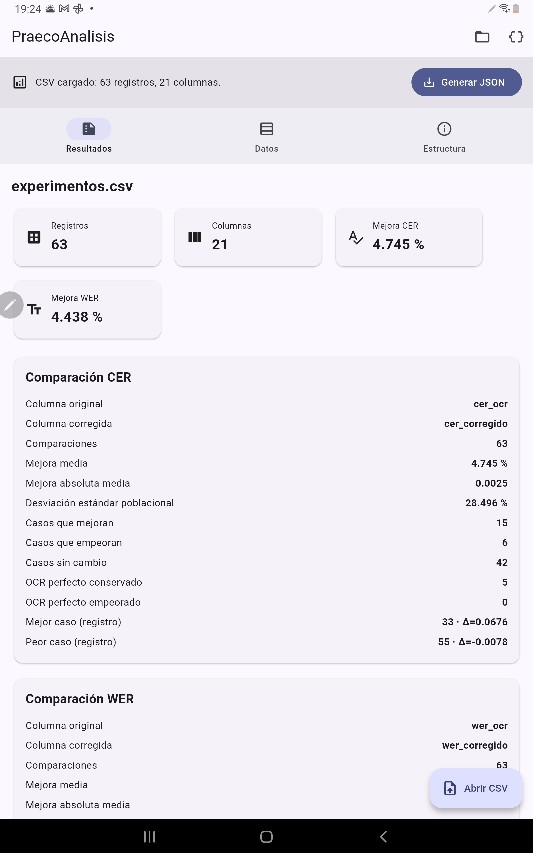
\includegraphics[
		width=\textwidth,
		height=0.39\textheight,
		keepaspectratio
		]{imagenes/16972.jpg}
		\caption{Resumen general y comparación de las métricas CER y WER.}
		\label{fig:praeco-analisis-1}
	\end{subfigure}
	\hfill
	\begin{subfigure}[t]{0.46\textwidth}
		\centering
		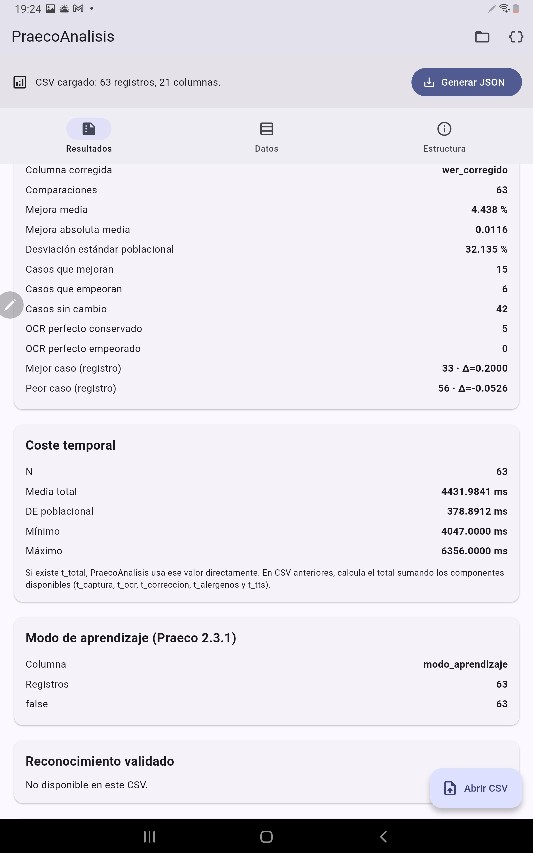
\includegraphics[
		width=\textwidth,
		height=0.39\textheight,
		keepaspectratio
		]{imagenes/16973.jpg}
		\caption{Evaluación del corrector y análisis del coste temporal.}
		\label{fig:praeco-analisis-2}
	\end{subfigure}
	
	\vspace{0.5cm}
	
	% =====================================================
	% SEGUNDA FILA
	% =====================================================
	
	\begin{subfigure}[t]{0.46\textwidth}
		\centering
		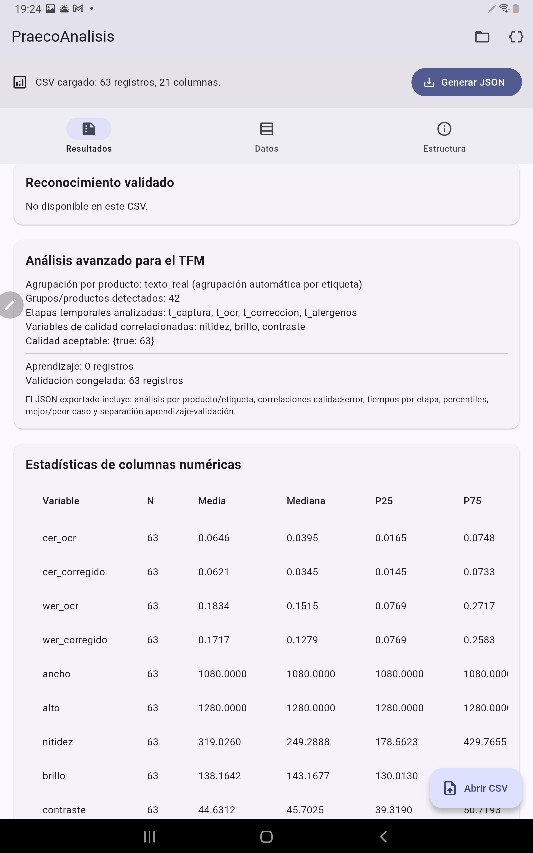
\includegraphics[
		width=\textwidth,
		height=0.39\textheight,
		keepaspectratio
		]{imagenes/16974.jpg}
		\caption{Análisis avanzado y estadísticos de las variables registradas.}
		\label{fig:praeco-analisis-3}
	\end{subfigure}
	\hfill
	\begin{subfigure}[t]{0.46\textwidth}
		\centering
		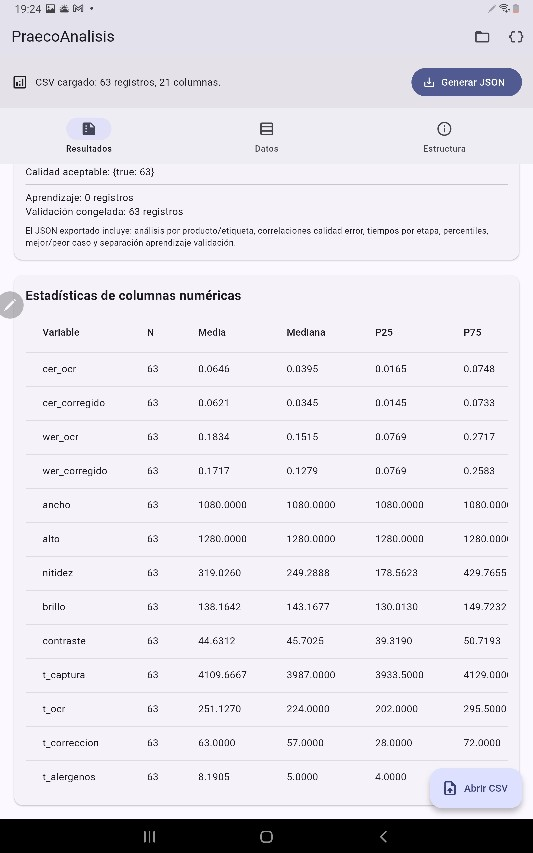
\includegraphics[
		width=\textwidth,
		height=0.39\textheight,
		keepaspectratio
		]{imagenes/16975.jpg}
		\caption{Estadísticos de calidad y tiempos de procesamiento.}
		\label{fig:praeco-analisis-4}
	\end{subfigure}
	
	\caption{Pantallas de ejemplo de Praeco Análisis.}
	
	\label{fig:praeco-analisis-pantallas}
\end{figure}

\newpage

% ------------------------------------------------
\section{Discusión de los resultados}
% ------------------------------------------------

Los resultados obtenidos a lo largo del desarrollo de Praeco muestran que la evaluación del corrector no puede reducirse únicamente a comprobar si los valores medios de CER o WER disminuyen. Aunque estas métricas permiten cuantificar de forma objetiva la precisión del reconocimiento, resulta igualmente necesario estudiar el comportamiento del corrector registro a registro, su estabilidad y, especialmente, su capacidad para conservar aquellas palabras que el OCR ya ha reconocido correctamente.

Debe tenerse en cuenta, además, que el fichero \texttt{experimentos.csv} se ha construido de forma incremental durante el desarrollo del proyecto. Los registros almacenados corresponden a distintas fases de análisis, ajuste y mejora de la aplicación. Paralelamente, durante las etapas en las que el aprendizaje se encontraba habilitado, se fue enriqueciendo el fichero \texttt{diccionario\_adaptativo.json} con vocabulario validado a partir de los experimentos realizados. Por tanto, el conjunto completo de registros refleja también la evolución del sistema y no debe interpretarse como un único ensayo realizado con una versión estática de Praeco.

Las primeras versiones del corrector mostraron que una estrategia excesivamente permisiva podía solucionar determinados errores del OCR y, simultáneamente, introducir sustituciones incorrectas sobre palabras que originalmente eran válidas. Esta situación explica que algunos experimentos presentasen mejoras locales mientras que las métricas globales permanecían prácticamente constantes o incluso empeoraban. Estos resultados fueron especialmente útiles durante el desarrollo, ya que permitieron identificar la necesidad de aumentar el carácter conservador del corrector.

Como consecuencia de este análisis se incorporaron progresivamente reglas de protección, criterios de confianza, control de conflictos y vocabulario adaptativo. El objetivo dejó de ser corregir el mayor número posible de palabras para pasar a modificar únicamente aquellas para las que existe evidencia suficiente de que se ha producido un error de reconocimiento.

El \texttt{diccionario\_adaptativo.json} constituye un elemento relevante en esta evolución. Su contenido representa vocabulario validado durante las fases de desarrollo y permite que términos encontrados previamente puedan ser reconocidos posteriormente como palabras válidas. De este modo se evita que el corrector sustituya innecesariamente términos correctos y se facilita la obtención de una salida \texttt{ocr\_corregido} más precisa. Conviene señalar que este mecanismo no modifica directamente el funcionamiento interno de Google ML Kit ni el texto OCR bruto, sino que actúa en la etapa posterior de corrección desarrollada específicamente en Praeco.

El análisis del conjunto formado por 63 registros, realizado con \texttt{modo\_aprendizaje = false}, permite evaluar el comportamiento del sistema utilizando los recursos lingüísticos previamente adquiridos pero manteniéndolos congelados durante la validación. En este conjunto, el CER medio pasa de 0.0646 para el OCR original a 0.0621 después de la corrección, mientras que el WER medio disminuye de 0.1834 a 0.1717. Praeco Análisis obtiene una mejora media del CER del 4.745\,\% y del WER del 4.438\,\%.

Sin embargo, esta mejora global no significa que todos los registros mejoren individualmente. En la comparación del CER, 15 registros mejoran, 6 empeoran y 42 permanecen sin cambios. Además, se conservan los cinco casos en los que el OCR era inicialmente perfecto, sin que el corrector introduzca errores en ellos. Estos resultados son coherentes con el criterio conservador adoptado: una proporción elevada de casos sin cambios no debe interpretarse necesariamente como una limitación, puesto que el objetivo es evitar modificaciones cuando no existe suficiente evidencia para realizarlas.

El análisis del WER conduce a una conclusión similar. La reducción de su valor medio indica que el corrector puede aportar una mejora global en el reconocimiento a nivel de palabra, pero siguen existiendo casos particulares en los que la corrección no produce ninguna modificación o puede introducir un empeoramiento. Por ello, el resultado agregado debe analizarse conjuntamente con el número de casos que mejoran, empeoran o permanecen inalterados.

El aprendizaje adaptativo tampoco debe interpretarse como un mecanismo de traducción o normalización automática al castellano. Su finalidad consiste en incorporar conocimiento validado del dominio. Las etiquetas comerciales pueden contener nombres propios, marcas, términos técnicos y vocabulario perteneciente a otros idiomas. Cuando estos términos aparecen realmente en el \textit{ground truth}, deben considerarse palabras válidas y conservarse. Un término extranjero correctamente reconocido no constituye por sí mismo un error de OCR.

Otro aspecto relevante es el coste temporal introducido por las diferentes etapas. Para el conjunto de 63 registros, Praeco Análisis obtiene un tiempo medio total de aproximadamente 4432~ms. La mayor parte corresponde al proceso de captura y selección de la imagen, con aproximadamente 4110~ms de media. El reconocimiento OCR requiere alrededor de 251~ms, mientras que la corrección presenta un tiempo medio próximo a 63~ms y la detección de alérgenos aproximadamente 8~ms. Estos resultados muestran que las etapas específicas de corrección y detección añadidas por Praeco representan una fracción reducida del tiempo total de procesamiento.

Desde el punto de vista funcional, este comportamiento resulta especialmente importante debido al objetivo asistencial de la aplicación. El texto corregido se utiliza posteriormente para la detección de términos asociados a alérgenos y para su reproducción mediante síntesis de voz. Una corrección incorrecta puede, por tanto, propagarse hacia las etapas posteriores. Esta circunstancia justifica que el sistema priorice la conservación de palabras válidas frente a una estrategia más agresiva orientada únicamente a maximizar el número de sustituciones.

Finalmente, la separación del sistema en Praeco Desarrollo, Praeco Usuario y Praeco Análisis ha permitido diferenciar claramente tres funciones. Praeco Desarrollo proporciona los mecanismos de experimentación, aprendizaje y generación de resultados; Praeco Usuario utiliza los recursos lingüísticos obtenidos sin necesidad de \textit{ground truth} ni aprendizaje durante el uso normal; y Praeco Análisis permite procesar los resultados experimentales, calcular estadísticos, comparar CER y WER, analizar el coste temporal y estudiar el comportamiento del corrector.

% ------------------------------------------------
\section{Ensayos exploratorios de captura rápida e iluminación asistida}

Después de la validación principal de 63 registros se desarrolló una versión de captura optimizada con una sola fotografía, control de linterna y mejora condicional. Los resultados de esta etapa constituyen \textbf{pruebas exploratorias posteriores}, no una ampliación de la muestra de validación del corrector ni un ensayo controlado de CLAHE.

En dos registros de la prueba con umbral de linterna 150 se obtuvieron los valores de la Tabla~\ref{tab:captura-rapida}. Las imágenes fueron aceptadas y el OCR corregido alcanzó CER y WER nulos en ambos casos.

\begin{table}[htbp]
\centering\small
\caption{Dos ensayos exploratorios de captura rápida con umbral de iluminación 150.}
\label{tab:captura-rapida}
\begin{tabular}{lrr}
\hline
\textbf{Indicador} & \textbf{Mejillones Galica} & \textbf{Don Simón}\\ \hline
Brillo medio & 132,93 & 163,73\\
Nitidez & 511,41 & 402,35\\
Contraste & 44,46 & 37,52\\
Tiempo de captura (ms) & 1842 & 1530\\
Tiempo OCR (ms) & 194 & 114\\
CER antes de corrección & 0,0172 & 0,0167\\
CER después de corrección & 0 & 0\\
WER después de corrección & 0 & 0\\ \hline
\end{tabular}
\end{table}

El tiempo medio de captura de estas dos observaciones fue 1686~ms, frente a los aproximadamente 4110~ms de captura media de la validación anterior. La diferencia descriptiva es de 2424~ms (aproximadamente un 59\,\%), pero \textbf{no puede interpretarse como una mejora causal demostrada}, porque los conjuntos de imágenes y las condiciones experimentales no son equivalentes y el alcance de los temporizadores debe comprobarse. El brillo de 132,93 corresponde a la imagen registrada y no prueba por sí solo el estado de la linterna durante la vista previa.

En ambos registros el OCR se realizó sobre la imagen original; por ello, \textbf{no se atribuye a CLAHE la reducción de CER o WER}. Para demostrar la aportación de esta técnica será necesario comparar, sobre las mismas capturas, OCR original frente a OCR con CLAHE, con el corrector y los recursos de aprendizaje congelados. También se requiere registrar el brillo previo, el estado de la linterna y el tiempo de estabilización para caracterizar el control de iluminación.

\section{Conclusiones del análisis experimental}
% ------------------------------------------------

Los resultados obtenidos durante las diferentes etapas de desarrollo y validación permiten extraer las siguientes conclusiones:

\begin{itemize}
	
	\item Las métricas CER y WER permiten cuantificar objetivamente tanto los errores producidos por el OCR como el efecto posterior del corrector desarrollado para Praeco.
	
	\item Las primeras versiones demostraron que una estrategia de corrección excesivamente permisiva puede introducir falsos positivos y empeorar palabras que originalmente habían sido reconocidas correctamente.
	
	\item La incorporación de reglas de protección, criterios de confianza y mecanismos de validación ha permitido evolucionar hacia una estrategia de corrección más conservadora.
	
	\item El aprendizaje adaptativo permite construir progresivamente un vocabulario específico a partir de información validada durante la fase de desarrollo. Este conocimiento queda almacenado principalmente en \texttt{diccionario\_adaptativo.json} y puede ser reutilizado posteriormente por el corrector.
	
	\item El fichero \texttt{experimentos.csv} refleja la evolución experimental de Praeco, puesto que se ha ido ampliando durante las diferentes etapas de análisis y mejora de la aplicación. Por esta razón, sus registros no deben interpretarse necesariamente como resultados obtenidos con una única versión estática del sistema.
	
	\item Los experimentos realizados con \texttt{modo\_aprendizaje = true} pertenecen a la fase de adquisición de conocimiento y no deben confundirse con una validación independiente del sistema.
	
	\item La utilización de \texttt{modo\_aprendizaje = false} permite congelar los recursos adquiridos y evaluar el comportamiento del corrector sin que los propios datos de validación modifiquen simultáneamente el sistema.
	
	\item En el conjunto analizado de 63 registros con aprendizaje desactivado se obtiene una mejora global de las métricas. El CER medio disminuye de 0.0646 a 0.0621 y el WER medio de 0.1834 a 0.1717, correspondientes a mejoras medias calculadas por Praeco Análisis del 4.745\,\% y del 4.438\,\%, respectivamente.
	
	\item La mejora global no implica una mejora individual en todos los casos. Para CER, 15 registros mejoran, 6 empeoran y 42 permanecen sin cambios. Los cinco casos con OCR inicialmente perfecto se conservan sin introducir errores, lo que constituye un indicador relevante del carácter conservador del corrector.
	
	\item La auditoría manual del \textit{ground truth} resulta imprescindible para que los valores obtenidos de CER y WER representen correctamente el error real del sistema.
	
	\item El vocabulario multilingüe, los nombres propios, las marcas y otros términos presentes legítimamente en las etiquetas deben conservarse y no considerarse automáticamente errores. El aprendizaje adaptativo no constituye un mecanismo de traducción.
	
	\item El análisis temporal muestra que el coste añadido específicamente por la corrección y la detección de alérgenos es reducido respecto al tiempo total de procesamiento. La mayor parte del tiempo corresponde al proceso de adquisición y selección de la imagen.
	
	\item La separación entre Praeco Desarrollo, Praeco Usuario y Praeco Análisis permite distinguir claramente las fases de experimentación y aprendizaje, utilización del asistente y evaluación de los resultados.
	
\end{itemize}

En conjunto, los resultados permiten concluir que el corrector de Praeco produce una mejora global moderada de las métricas CER y WER en el conjunto de validación analizado, aunque dicha mejora no se produce de manera uniforme en todos los registros. Este comportamiento confirma la conveniencia de utilizar una estrategia conservadora, en la que una palabra únicamente se modifica cuando existe evidencia suficiente para realizar la corrección.

La evolución del \texttt{diccionario\_adaptativo.json} permite incorporar conocimiento validado durante el desarrollo y reutilizarlo posteriormente sin modificar los recursos durante la fase de validación. La combinación de aprendizaje previo, congelación de los recursos y evaluación posterior proporciona una metodología más rigurosa que la utilización simultánea de aprendizaje y validación sobre los mismos datos.

Por último, el desarrollo de Praeco no se limita al reconocimiento óptico de caracteres, sino que integra adquisición y selección automática de imágenes, OCR, corrección léxica, aprendizaje adaptativo, detección de términos asociados a alérgenos, síntesis de voz y herramientas específicas para la evaluación experimental. Los resultados obtenidos muestran que esta arquitectura puede ejecutarse en un dispositivo móvil con un coste adicional reducido para las etapas de corrección y detección, manteniendo como criterio fundamental la conservación del texto correctamente reconocido.


\chapter{Conclusiones y trabajos futuros}

% ------------------------------------------------
\section{Conclusiones}
% ------------------------------------------------

El desarrollo realizado en este Trabajo Fin de Máster ha permitido diseñar, implementar y evaluar un asistente móvil orientado a facilitar el acceso a la información textual presente en etiquetas de productos a personas con discapacidad visual. El sistema desarrollado, denominado Praeco, combina técnicas de visión artificial, reconocimiento óptico de caracteres, procesamiento lingüístico, aprendizaje adaptativo, detección de términos asociados a alérgenos y síntesis de voz dentro de una aplicación ejecutable sobre dispositivos Android convencionales.

El trabajo ha evolucionado desde un prototipo centrado fundamentalmente en la captura y reconocimiento OCR hasta un ecosistema formado por tres aplicaciones diferenciadas: \textit{Praeco Desarrollo}, \textit{Praeco Usuario} y \textit{Praeco Análisis}. Esta separación permite distinguir claramente las tareas de experimentación y aprendizaje, el funcionamiento normal del asistente y el análisis posterior de los resultados.

Praeco Desarrollo incorpora la instrumentación necesaria para evaluar el sistema mediante \textit{ground truth}, calcular las métricas CER y WER, registrar los tiempos de ejecución, almacenar las variables asociadas a la calidad de imagen y realizar aprendizaje adaptativo. Praeco Usuario utiliza los recursos obtenidos durante el desarrollo, pero elimina los mecanismos de evaluación y aprendizaje que no son necesarios durante el funcionamiento normal. Finalmente, Praeco Análisis permite procesar los ficheros experimentales y obtener automáticamente estadísticas sobre las métricas de reconocimiento, comportamiento del corrector, calidad de imagen y coste temporal.

Uno de los resultados más relevantes del trabajo ha sido comprobar que la corrección posterior al OCR debe realizarse de forma conservadora. Las primeras versiones mostraron que una estrategia excesivamente permisiva podía corregir determinados errores y, al mismo tiempo, modificar palabras que originalmente habían sido reconocidas correctamente. Como consecuencia, el corrector evolucionó incorporando reglas de protección, distancia de Levenshtein, criterios fonéticos, umbrales dependientes de la longitud de las palabras, criterios de confianza y vocabulario adaptativo.

El aprendizaje adaptativo permite incorporar progresivamente vocabulario validado durante la fase de desarrollo. Este conocimiento se almacena principalmente

 en \texttt{diccionario\_adaptativo.json} y puede reutilizarse posteriormente para reconocer como válidos términos previamente aprendidos. Este mecanismo no modifica el funcionamiento interno de Google ML Kit ni el OCR bruto, sino que mejora la etapa posterior de corrección y contribuye a obtener un texto \texttt{ocr\_corregido} más preciso.

Debe señalarse que el fichero \texttt{experimentos.csv} se ha construido progresivamente durante las distintas etapas de desarrollo, análisis y mejora de Praeco. Por este motivo, el conjunto completo de registros refleja también la evolución del sistema y de los recursos lingüísticos empleados. Durante las fases con aprendizaje activo se fue enriqueciendo el \texttt{diccionario\_adaptativo.json}, mientras que en la validación final los recursos fueron congelados mediante \texttt{modo\_aprendizaje = false}, evitando que los propios datos utilizados para validar el sistema modificasen simultáneamente el conocimiento adquirido.

Los resultados obtenidos en el conjunto de 63 registros analizado con los recursos congelados muestran una mejora global moderada después de aplicar el corrector. El CER medio disminuye de 0.0646 a 0.0621 y el WER medio de 0.1834 a 0.1717. Praeco Análisis calcula una mejora media del CER del 4.745\,\% y del WER del 4.438\,\%.

Esta mejora global no se produce de forma uniforme en todos los experimentos. En el análisis del CER, 15 registros mejoran, 6 empeoran y 42 permanecen sin cambios. Asimismo, los cinco registros en los que el OCR inicial era perfecto se conservan sin introducir errores adicionales. Este comportamiento resulta coherente con la estrategia conservadora adoptada: cuando el sistema no dispone de evidencia suficiente para realizar una sustitución, resulta preferible conservar el término reconocido originalmente.

La auditoría del \textit{ground truth} ha resultado igualmente fundamental para la evaluación experimental. CER y WER únicamente proporcionan resultados fiables cuando el texto utilizado como referencia representa fielmente el contenido de la etiqueta. Este proceso permitió además comprobar la existencia legítima de nombres comerciales, nombres propios y términos pertenecientes a diferentes idiomas. Por tanto, el aprendizaje adaptativo no debe interpretarse como un mecanismo de traducción al castellano: una palabra extranjera presente realmente en la etiqueta constituye un término válido y debe conservarse.

Otro resultado relevante corresponde al análisis temporal. Para los 63 registros evaluados se obtiene un tiempo medio total de aproximadamente 4432~ms. La mayor parte corresponde a la adquisición y selección de la imagen, con aproximadamente 4110~ms, mientras que el reconocimiento OCR requiere alrededor de 251~ms. La corrección presenta un coste medio próximo a 63~ms y la detección de términos asociados a alérgenos aproximadamente 8~ms. Por tanto, las etapas específicas añadidas por Praeco después del OCR representan una fracción reducida del tiempo global de procesamiento.

Como evolución posterior a la validación principal, se ha incorporado una estrategia de captura única con evaluación previa, iluminación auxiliar continua y preprocesamiento condicional mediante CLAHE. Dos ensayos exploratorios muestran tiempos de captura de 1842 y 1530~ms, pero no constituyen una validación controlada de la mejora ni permiten atribuir a CLAHE un incremento de precisión.

En conjunto, los resultados obtenidos permiten concluir que Praeco constituye un prototipo funcional capaz de integrar en un dispositivo móvil las principales etapas necesarias para capturar una etiqueta, seleccionar una imagen adecuada, reconocer su contenido textual, aplicar una corrección conservadora, identificar determinados términos asociados a alérgenos y comunicar el resultado mediante síntesis de voz.

% ------------------------------------------------
\section{Aportaciones principales del trabajo}
% ------------------------------------------------

Las principales aportaciones realizadas durante el desarrollo del proyecto pueden resumirse en los siguientes puntos:

\begin{itemize}[noitemsep]
	
	\item Desarrollo de una aplicación móvil accesible basada en Flutter y orientada a personas con discapacidad visual.
	
	\item Implementación inicial de adquisición y selección entre tres fotografías, posteriormente optimizada mediante evaluación de fotogramas en vista previa y captura automática única, con iluminación auxiliar estabilizada.
	
	\item Incorporación de preprocesamiento condicional de imagen mediante CLAHE y ajustes de iluminación, con conservación y comparación visual de la fotografía original y la procesada.

\item Definición de una región de interés (\textit{Region of Interest}, ROI) para reducir la información innecesaria y concentrar el reconocimiento sobre la zona relevante de la etiqueta.
	
	\item Integración de Google ML Kit como motor de reconocimiento óptico de caracteres.
	
	\item Desarrollo de un sistema propio de filtrado y reconstrucción del texto obtenido mediante OCR.
	
	\item Implementación de un corrector léxico híbrido basado en distancia de Levenshtein, información fonética, diferencias de longitud, criterios de confianza y mecanismos de protección de términos válidos.
	
	\item Desarrollo de un mecanismo de aprendizaje incremental basado en los errores observados durante los experimentos y en la incorporación de vocabulario validado al \texttt{diccionario\_adaptativo.json}.
	
	\item Implementación de mecanismos específicos para proteger números, unidades, palabras cortas, nombres propios, marcas y vocabulario multilingüe presente legítimamente en las etiquetas.
	
	\item Detección automática de términos asociados a diferentes categorías de alérgenos y consideración de expresiones de ausencia o negación, como ``sin gluten'', para reducir falsos positivos.
	
	\item Integración de síntesis de voz para comunicar al usuario el texto reconocido y las advertencias obtenidas.
	
\end{itemize}
	


% ------------------------------------------------
\section{Trabajos futuros}
% ------------------------------------------------

Los resultados obtenidos permiten identificar varias líneas de continuación que pueden mejorar tanto la robustez técnica de Praeco como la validez externa de su evaluación.

\begin{itemize}[noitemsep]
    \item \textbf{Ampliación del corpus experimental.} Incrementar el número y la diversidad de etiquetas, condiciones de iluminación, tipografías, materiales de envase y dispositivos permitiría caracterizar con mayor precisión el comportamiento del sistema y estudiar su capacidad de generalización.

    \item \textbf{Evaluación con usuarios.} La validación realizada en este TFM se centra principalmente en métricas técnicas. Un trabajo posterior debería incorporar pruebas de usabilidad y accesibilidad con personas con discapacidad visual, evaluando aspectos como facilidad de captura, comprensión de los mensajes, tiempos percibidos y utilidad en situaciones reales.

    \item \textbf{Mejora del tratamiento multilingüe.} Las etiquetas comerciales pueden contener nombres propios y términos en distintos idiomas. Resulta de interés ampliar los mecanismos de protección e identificación lingüística para reducir correcciones indebidas sin convertir el corrector en un sistema de traducción.

    \item \textbf{Evaluación de mecanismos contextuales.} Los recursos basados en n-gramas se encuentran disponibles en el proyecto, pero la corrección contextual no forma parte de la ruta activa evaluada en los 63 registros finales. Una línea futura consiste en activar y validar experimentalmente este mecanismo mediante un estudio de ablación que permita cuantificar su aportación independiente.

    \item \textbf{Ampliación de la detección de alérgenos.} El módulo actual identifica términos asociados a determinadas categorías y expresiones de negación. Su evolución debería contemplar vocabulario más amplio, variantes lingüísticas y una validación específica sobre etiquetado alimentario. En cualquier caso, esta función debe mantenerse como ayuda informativa y no como certificación de seguridad alimentaria.

    \item \textbf{Optimización de la adquisición.} Dado que la captura y selección de la imagen concentra la mayor parte del tiempo total de procesamiento, la versión optimizada debe validarse con un corpus ampliado y condiciones controladas, comparando el tiempo extremo a extremo y la robustez de la activación de la linterna.

    \item \textbf{Evaluación específica de CLAHE.} Realizar un ensayo de ablación con las mismas imágenes, sin mejora, con CLAHE y con ajustes de brillo; medir CER, WER, latencia y posibles empeoramientos, manteniendo congelado el corrector.

    \item \textbf{Comparación entre dispositivos y motores OCR.} La evaluación en diferentes terminales Android y la comparación controlada con otros motores de reconocimiento permitirían determinar qué parte del rendimiento depende de la plataforma y qué parte corresponde específicamente a las etapas desarrolladas en Praeco.
\end{itemize}

Estas líneas permitirían evolucionar Praeco desde el prototipo funcional y experimental desarrollado en este TFM hacia una herramienta asistencial más robusta, manteniendo como principio metodológico la separación entre aprendizaje, validación y uso final.



\newpage
\addcontentsline{toc}{chapter}{Bibliografía y referencias} %Para 

\bibliography{bibliografia}
% \printbibliography
\nocite{*}
\glsaddall


% Apéndices
\appendix
% ============================================================
% APÉNDICE A - SOFTWARE DESARROLLADO
% ============================================================
\chapter{Software desarrollado}
\label{ap:software}

\section{Introducción}
Como parte de este Trabajo Fin de Máster se ha desarrollado \textit{Praeco}, un sistema software orientado a facilitar el acceso a la información textual presente en el etiquetado de productos mediante técnicas de visión artificial, reconocimiento óptico de caracteres y síntesis de voz. La versión final se organiza en tres aplicaciones independientes: \textbf{Praeco Desarrollo}, \textbf{Praeco Usuario} y \textbf{Praeco Análisis}.

\section{Repositorio y versión de referencia}
El código fuente correspondiente a la versión final de Praeco se encuentra disponible públicamente en el repositorio GitHub del proyecto:
\begin{center}
\url{https://github.com/fjlopezlp-beep/Asistente-Discapacidad-Visual}
\end{center}
La versión utilizada como referencia para la entrega final se identifica mediante la etiqueta \texttt{v2.3.1-TFM} y la \textit{release} \textbf{Praeco v2.3.1 -- TFM}. Las tres aplicaciones se identifican con la versión \texttt{2.3.1+1}.

\section{Estructura del repositorio}
El repositorio separa las tres aplicaciones en los directorios \texttt{Praeco\_Desarrollo}, \texttt{Praeco\_Usuario} y \texttt{Praeco\_Analisis}. Cada aplicación conserva su propio código fuente, recursos, configuración Android y ficheros \texttt{pubspec.yaml} y \texttt{pubspec.lock}. No se incluyen cachés de Flutter, resultados de compilación ni configuraciones locales del entorno de desarrollo.

\section{Praeco Desarrollo}
Praeco Desarrollo corresponde a la aplicación utilizada durante las fases de implementación, aprendizaje, experimentación y validación. Integra la adquisición y evaluación de calidad de la imagen, selección de la región de interés, OCR mediante Google ML Kit, filtrado y reconstrucción del texto, corrección léxica, recursos de aprendizaje adaptativo, detección de términos asociados a alérgenos, síntesis de voz y evaluación mediante CER y WER. Durante la validación final, los recursos de aprendizaje se mantienen congelados.

\section{Praeco Usuario}
Praeco Usuario constituye la versión destinada al funcionamiento normal del asistente. No requiere la introducción de \textit{ground truth} ni realiza el cálculo de CER y WER durante su utilización. Emplea los recursos lingüísticos previamente obtenidos y congelados, manteniendo estable el comportamiento del corrector.

\section{Praeco Análisis}
Praeco Análisis es una aplicación independiente destinada al tratamiento estadístico de los resultados experimentales. Permite estudiar CER, WER, comportamiento del corrector, variables de calidad de imagen y tiempos de procesamiento. No necesita los diccionarios empleados por el corrector, puesto que analiza resultados previamente obtenidos y no ejecuta de nuevo el proceso de corrección.

\section{Requisitos de compilación}
Cada aplicación dispone de su propio fichero \texttt{pubspec.yaml}. Una vez instalado y configurado Flutter, las dependencias pueden recuperarse mediante \texttt{flutter pub get}; la aplicación puede ejecutarse con \texttt{flutter run} y puede generarse un APK de distribución mediante \texttt{flutter build apk --release}.

\section{Reproducibilidad}
La combinación del código fuente, los recursos necesarios, la definición y bloqueo de dependencias, la etiqueta Git específica y la \textit{release} asociada permite identificar de forma inequívoca el estado del software utilizado como referencia para el Trabajo Fin de Máster.

\section{Datos generados durante la experimentación}
Durante la ejecución de Praeco Desarrollo se utiliza el directorio \texttt{TFM\_OCR} del dispositivo Android para almacenar datos generados durante los experimentos. Este directorio constituye un espacio de trabajo y no forma parte del código fuente necesario para compilar la aplicación.

Para garantizar la trazabilidad de la evaluación presentada en esta memoria se ha preparado un conjunto de validación independiente, publicado como archivo adicional de la \textit{release} \texttt{v2.3.1-TFM}. El archivo \texttt{Praeco\_Dataset\_Validacion\_TFM.zip} contiene el fichero de resultados correspondiente a 63 registros de validación con el aprendizaje desactivado, las imágenes asociadas y la información de trazabilidad disponible.

\section{Disponibilidad del software}
La versión de referencia utilizada para la entrega de este Trabajo Fin de Máster es \textbf{Praeco v2.3.1 -- TFM}, identificada mediante la etiqueta \texttt{v2.3.1-TFM} en el repositorio indicado anteriormente.





\end{document}